
\subsection{Analysis procedure}

Measurements in this analysis are carried out by considering correlations between high-$p_{\rm T}$ jets and tracks in PbPb and pp collisions.  Jets are selected within $\eta < 1.6$ and $p_{\rm T}$ above a particular threshold.  For each jet, the relative separation in pseudorapidity ($\Delta\eta = \eta_{\rm track} - \eta_{jet}$) and azimuth ($\Delta\eta = \phi_{\rm track} - \phi_{jet}$) is measured between the jet and all charged-hadron tracks within $\eta < 2.4$.  For each jet-track pair, these measurements are recorded in a two-dimensional $\Delta\eta - \Delta\phi$ correlation in a particular track transverse momentum ($p_{\rm T}^{\rm trk}$) and centrality class.  Each correlation is normalized by dividing by the number of jets in the sample ($N_{\rm jets}$), resulting in a signal pair distribution, $S(\Delta\eta,\Delta\phi)$, that gives the per-jet yield of tracks and their relative distance from the jet:

  \begin{equation}
  \label{eq:signal}
  S(\Delta\eta,\Delta\phi) = \frac{1}{N_{\rm jets}}\frac{\rm d^{2} N^{\rm same}}{\rm d\Delta\eta d\Delta\phi}.
  \end{equation}

This procedure results in a two dimensional measurement of the distribution of charged tracks with respect to the jet axis.  The same procedure may also be repeated, weighting each track by its $p_{\rm T}^{\rm trk}$, in order to obtain a distribution of transverse momentum with respect to the jet axis.  These particle density and $p_{\rm T}^{\rm trk}$ correlations form the basis for all results discussed in this analysis.  From this point, several additional corrections and other steps are necessary to isolate jet-related effects from long range and uncorrelated backgrounds.  These additional steps are as follows: 
\begin{itemize}
\item A correction for jet-track pair acceptance effects;
\item Separation of correlations into short-range jet peaks and and long range components;
\item Monte Carlo-based corrections for biases related to jet reconstruction.
\end{itemize}
After these steps, a range of different observables may be extracted to characterize the multiplicity and distribution of tracks and $p_{\rm T}^{\rm trk}$ at both small and large angles from the jet axis.  

\clearpage

\subsection{Jet-track correlation pair-acceptance correction}

This analysis considers $\Delta\eta$ jet-track separations as large as $\Delta\eta = 2.5$.  With finite $\eta$ acceptance for both jets and tracks ($|\eta_{\rm jet}| < 1.6$ and $|\eta_{\rm track}| < 2.4$, tracks that fall within $\Delta\eta = 2.5$ of a jet may be outside the tracking acceptance.  This pair acceptance effect results in trapezoidal correlations that fall with rising $|\Delta\eta|$ as tracks are ``lost'' outside of the acceptance.  This effect is purely geometric, and may be corrected by reproducing this pair acceptance geometry.  This is done by creating a ``mixed event'' correlation in which jets in the sample are correlated to tracks within $|\eta| < 2.4$ from randomly selected events in a minimum bias PbPb sample, matched in vertex-$z$ position (within 0.5 cm) and centrality (within 2.5\%).  This reproduces the pair acceptance geometry from the signal correlations: 
  
  \begin{equation}
  \label{eq:background}
  ME(\Delta\eta,\Delta\phi) = \frac{1}{N_{\rm jets}}\frac{\rm d^{2}N^{\rm mix}}{\rm d\Delta\eta d\Delta\phi},
  \end{equation}
  is constructed to account for pair-acceptance effects, with $N^{\rm mix}$ denoting the number of mixed-event jet-track pairs.  The mixed event correction is normalized to unity at $\Delta\eta$=0, where the jet and track are colinear in $\eta$ and therefore have perfect pair acceptance, with the normalization factor $ME(0,0)$.  Dividing the signal correlation $S(\Delta\eta,\Delta\phi)$, defined in Equation~\ref{eq:signal}, by this normalized mixed event correlation $ME(\Delta\eta,\Delta\phi)$/$ME(0,0)$ yields the corrected per-jet correlated yield distribution, as illustrated in Figure~\ref{fig:ME_corr}: 

  \begin{equation}
  \label{2pcorr_incl}
  \frac{1}{N_{\rm jets}}\frac{\rm d^{2} N}{\rm d\Delta\eta\, \rm d\Delta\phi}
  = \frac{ME(0,0)}{ME(\Delta\eta,\Delta\phi)}\times S(\Delta\eta,\Delta\phi).
  \end{equation}
  
\begin{figure}[ht!] 
\begin{center} 
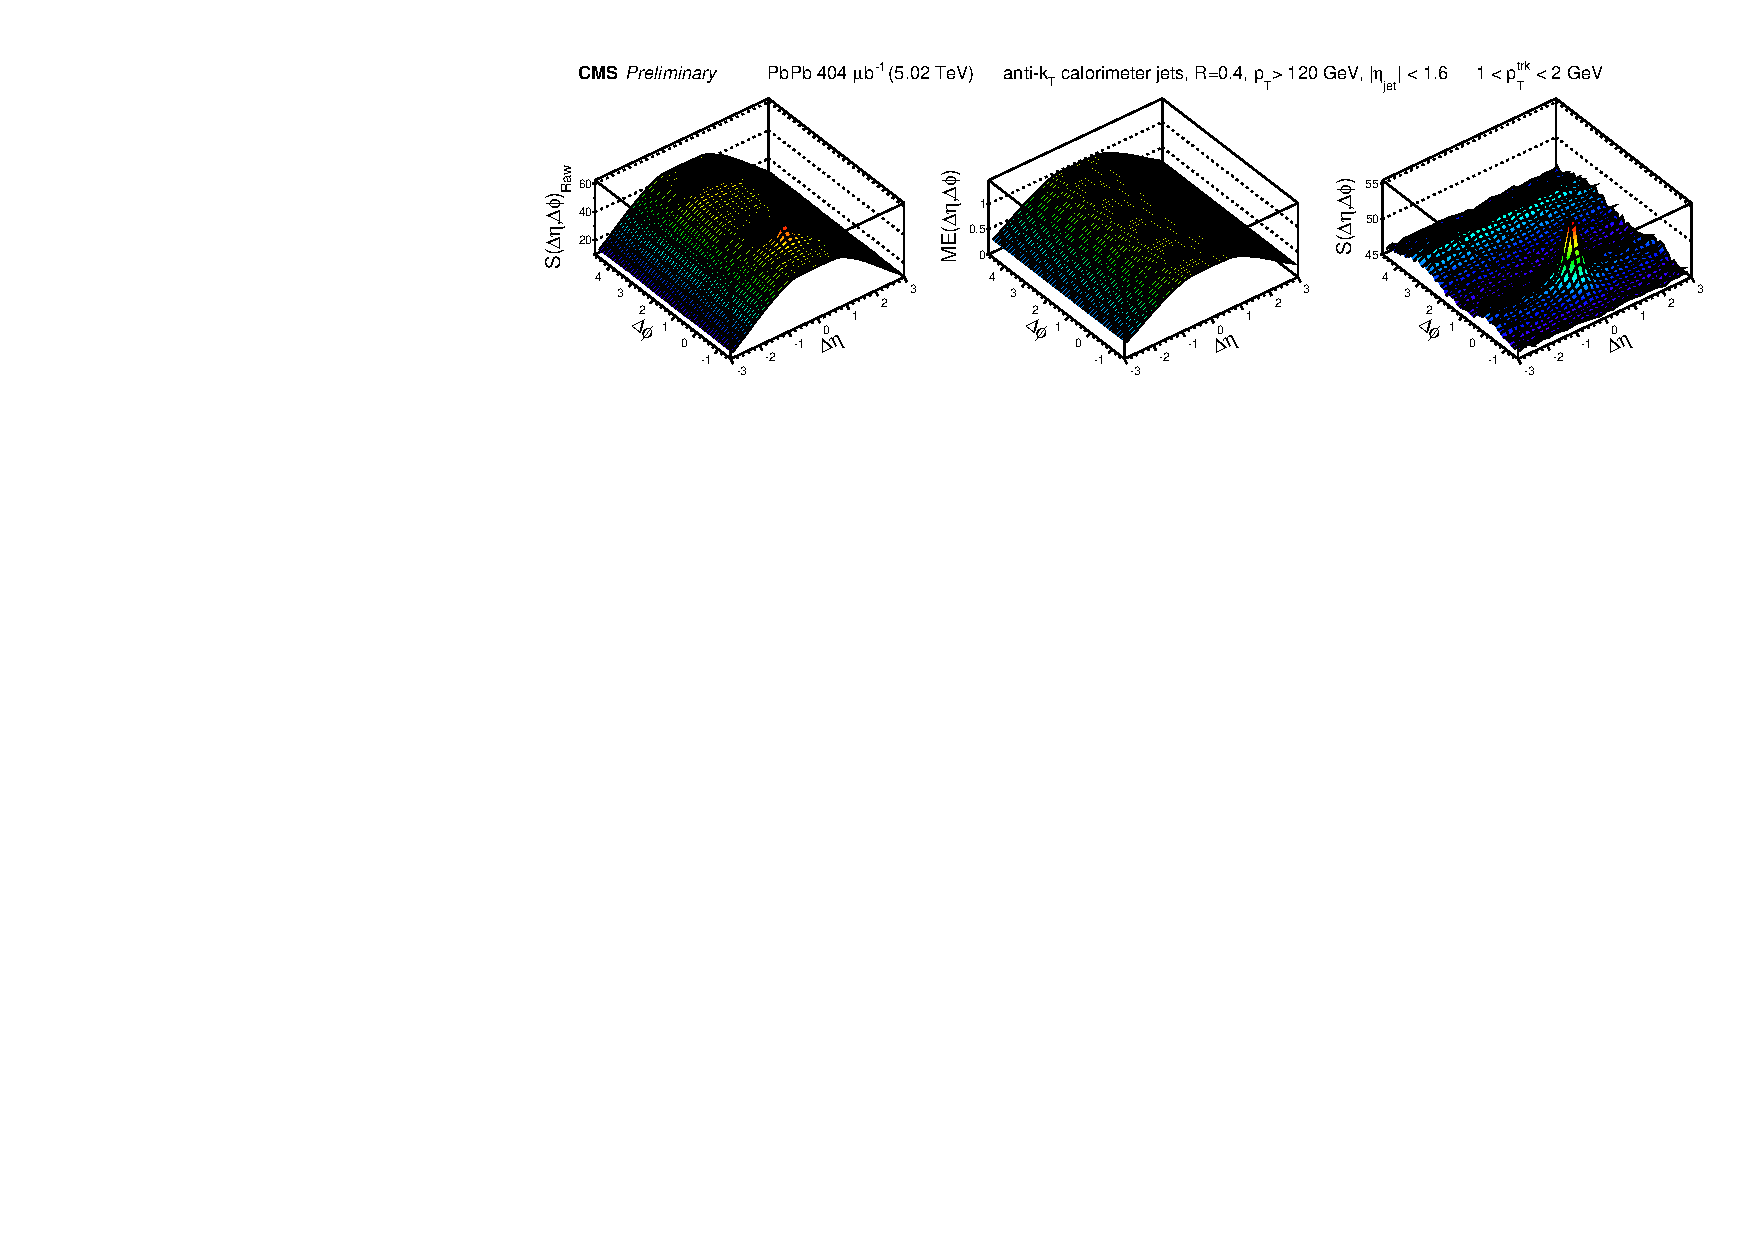
\includegraphics[width=0.99\textwidth]{figures/Results/ME_Correction.pdf}
\caption[Illustration of the pair-acceptance correction procedure]{Illustration of the pair-acceptance correction procedure:  left panel shows signal correlation $S(\Delta\eta,\Delta\phi)$, and center panel shows mixed event correlation $ME(\Delta\eta,\Delta\phi)$.  Dividing the signal correlation by the normalized mixed event correlation yields the corrected per-jet correlated yield distribution shown in the right panel.}
\label{fig:ME_corr}
\end{center} 
\end{figure} 

  
\subsection{Separation of correlations into long range and short-range components}
\label{sec:bkg_sub}

After correlations are corrected for pair-acceptance effects, in each correlation we are left with a well-defined jet peak sitting at $\Delta\eta = 0$, $\Delta\phi = 0$ on top of a large combinatoric and long range correlated background.  For most measurements, it is necessary to isolate this jet peak in order to distinguish jet-related effects from eventwise correlations.   In order to achieve this, we note that the long range correlation is independent of $\Delta\eta$ at distances larger than $\Delta\eta = 1.5$ from the jet.  This ``sideband'' region ($1.5 < |\Delta\eta| < 3.0$) is used to model the underlying event, capturing both the level of the combinatoric background in the event, and also the long range ``flow'' correlations in the event.  The assumption of rapidity--independence of the flow harmonics is based on the CMS study~\cite{v2_HIN_11_012}, which shows no appreciable variation of the elliptic flow for charged particles above 1~GeV in the pseudorapidity interval of $\Delta\eta < 3.0$ relevant for this study.  As long range correlations depend only on $\Delta\phi$, the sideband region is projected into $\Delta\phi$ to obtain a one-dimensional model of the underlying event.   To subtract this long range correlation in 2D, this distribution may be either directly re-propagated into $\Delta\phi$ (as shown in Figure~\ref{fig:BG_sub1}), or may be fit in $\Delta\phi$ before repropagation in a smoothing procedure as shown in Fig.~\ref{fig:BG_sub2}.  When aiming to simply remove the long range correlated background, we fit long range correlations function modeling harmonic flow plus a term to capture the (Gaussian or sharper) ``away-side'' peak opposite the jet in relative azimuth:  

\begin{equation}
\label{eq:bkg_fit_as}
B(\Delta\phi) = B_{0}(1+2V_{\rm1}\cos{(\Delta\phi)}+2V_{\rm 2}\cos{(2\Delta\phi)}+2V_{\rm 3}\cos{(3\Delta\phi)})+A_{\rm AS}\exp{\bigg(-\bigg(\frac{|\Delta\phi-\pi|}{\alpha}\bigg)^{\beta} \bigg) },
\end{equation}

\noindent In this case, the fit is performed only as a smoothing procedure to model the background under the near-side jet peak.; as only the jet peak within $|\Delta\phi|<\frac{\pi/}{2}$ is studied, the fit to the away-side peak is not relevant to the analysis.  Furthermore, no physics conclusions can be extracted from the $V_{n}$ terms in this fit, which are used only to establish a reasonable functional form for smooth modeling of the background distributions.  

\begin{figure}[t!] 
\begin{center} 
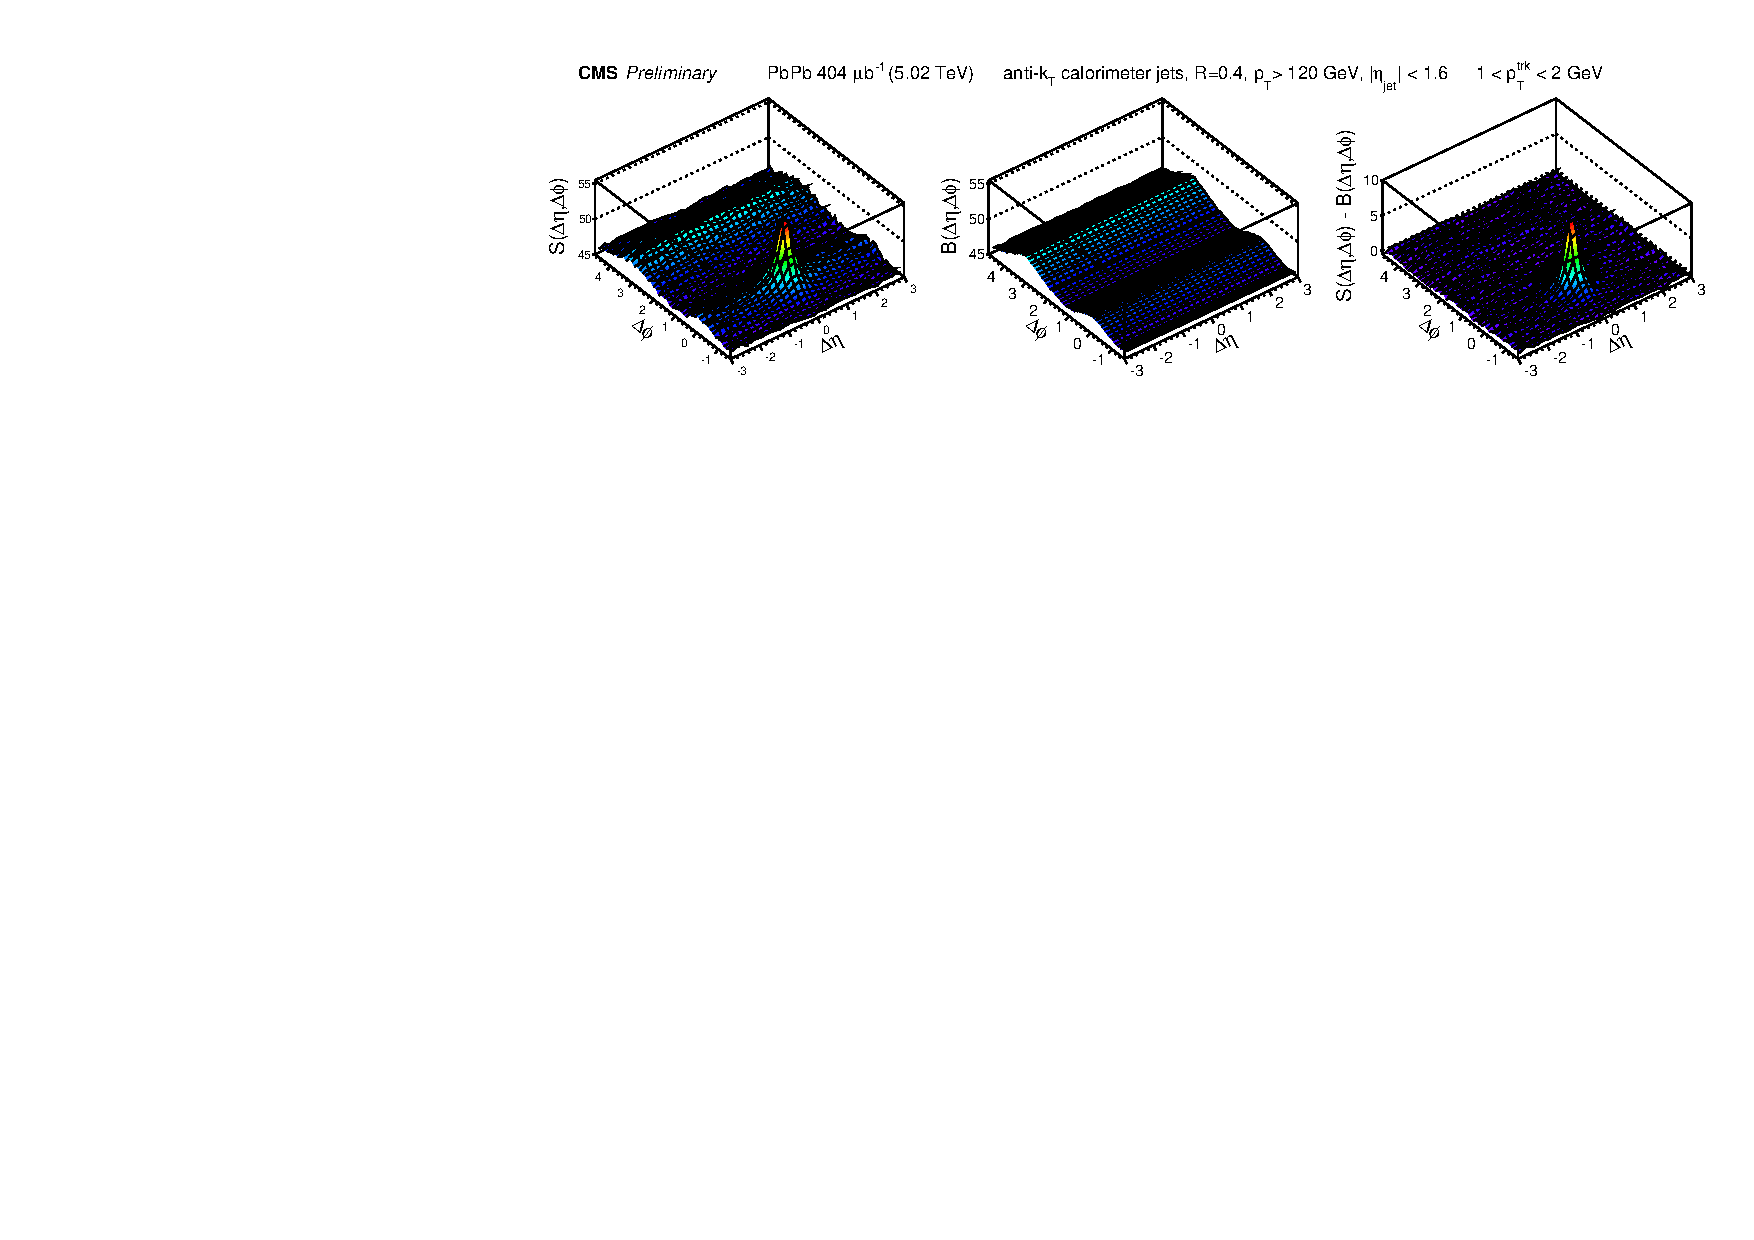
\includegraphics[width=0.99\textwidth]{figures/Results/Background_Subtraction.pdf}
\caption[Illustration of the event decomposition procedure without $\Delta\phi$ fitting]{Illustration of the event decomposition procedure without $\Delta\phi$ fitting:  left panel shows the acceptance-corrected correlation, middle panel shows the projected and re-propagated long range distribution, and right panel shows the background-subtracted jet peak.}
\label{fig:BG_sub1}
\end{center} 
\end{figure}

\begin{figure}[hbt] 
\begin{center} 
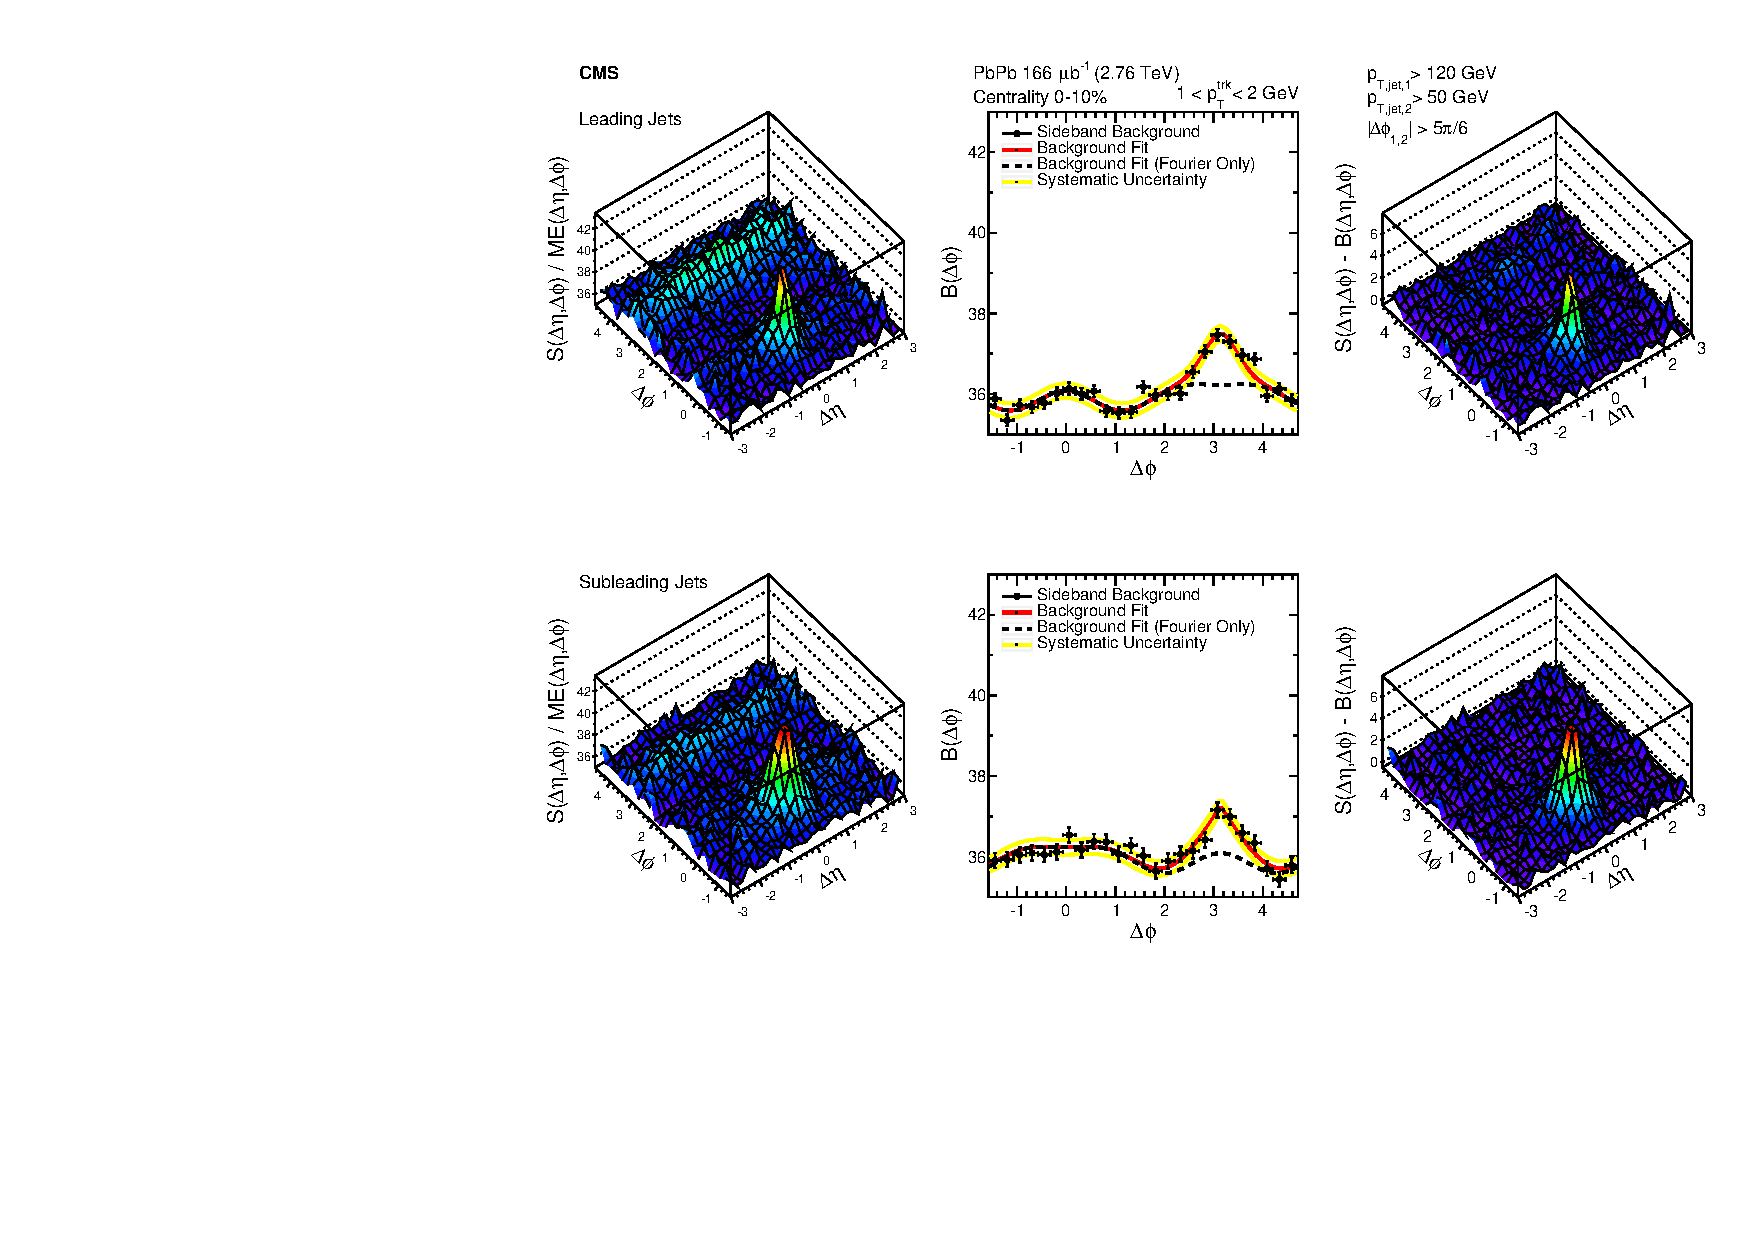
\includegraphics[width=0.99\textwidth]{figures/Results/PAS_Figure_2_TrkPt1_TrkPt2.pdf}
\caption[Illustration of the event decomposition procedure with $\Delta\phi$ fitting]{Illustration of the event decomposition procedure with $\Delta\phi$ fitting:  left panel shows the acceptance-corrected correlation, middle panel shows the projected and fit long range distribution, and right panel shows the background-subtracted jet peak.}
\label{fig:BG_sub2}
\end{center} 
\end{figure}


The long range correlations in the underlying event are in themselves interesting objects of study, however, as they contain information about the collective behavior of particles in the event as a whole, and the extent to which the distribution of high-$p_{\rm T}$ jets in the event couple to this collective flow.  To further study the long range correlations, we may apply the well-established harmonic flow decomposition method used to study two-particle correlations~\cite{Chatrchyan:2012wg} to correlations between jets and tracks.  In dijet studies, more accurate information about long range flow correlations can furthermore be obtained by making use of the fact that for our dijet selection and a given value of $\Delta\eta$ the region $-\frac{\pi}{2}<\Delta\phi<\frac{\pi}{2}$ of the leading correlation is by definition equivalent to the region $\frac{\pi}{2}<\Delta\phi<3\frac{\pi}{2}$ of the subleading correlation.  This provides a full $2\pi$ distribution of the long range correlated underlying event under both the leading and subleading jet peaks.  We can then perform a single fit to the combined background.  Here we fit with harmonic flow terms only:  

\begin{equation}
\label{eq:bkg_fit_dijet}
B(\Delta\phi)^{\rm Dijet} = B_{0}(1+2V_{\rm1}\cos{(\Delta\phi)}+2V_{\rm 2}\cos{(2\Delta\phi)}+2V_{\rm 3}\cos{(3\Delta\phi)}),
\end{equation}

\noindent In this fit, we find that terms through $\rm V_{3}$ are necessary to describe the low-$p_{\rm T}$, central background, while at higher-$p_{\rm T}$ only $\rm V_{1}$, $\rm V_ {2}$.  From this combined fit, we extract parameters $\rm V_{1}$, $\rm V_ {2}$, and $\rm V_{3}$.  Then, to better constrain the background under the signal and minimize the effects of random background fluctuations, we apply the factorization relation of overall Fourier harmonic $\rm V_{2} = v_{2}^{jet} \times v_{2}^{trk}$~\cite{Aamodt:2011by, Chatrchyan:2011eka}. The values of $\rm v_{2}^{trk}$ for charged particles are determined in Ref.~\cite{Chatrchyan:2012wg}, while the fit parameter $\rm v_{2}$ is expected to be independent of  $p_{\rm T}^{\rm trk}$ ranges for a given centrality class.  The average value of $\rm v_{2}^{jet}$ from each $p_{\rm T}^{\rm trk}$ range is calculated, and used to fix the $\rm V_{2}$ parameter on the second iteration of the fit.  Both the combined dijet fit with $B(\Delta\phi)^{\rm Dijet}$ and the final $B(\Delta\phi)$ fits are shown in Appendix~\ref{app:bkg_fits}.  Through this process, we characterize the underlying event and note that the distribution of jets as well as tracks couples to the flow modulation of the underlying event.  This has immediate consequences for studies of momentum balance between leading and subleading hemispheres of the event:  as there are non-zero contributions from odd harmonics to the long-range correlated backgrounds, we cannot expect flow cancellation when directly subtracting hemishpere $p_{\rm T}^{trk}$ distributions.  

For jet peak studies the underlying event is a background to subtracted to isolate jet peaks.  After this is done, either by direct subtraction or by subtracting the fit and re-propagated background, we are left with isolated 2D jet peaks.  Before extracting observables, we must carefully consider and correct for reconstruction biases affecting these correlated yields.  Before correlations are constructed, both tracks and jets are corrected for detector efficiencies and other reconstruction effects, as discussed in detail in Sec.~\ref{sec:Tracks} and Sec.~\ref{sec:Jets}, respectively.  There are two additional effects, however, in which jet biases are coupled to the multiplicity of low-$p_{\rm T}$ tracks:  a bias against reconstructing jets with soft fragmentation that arises from nonlinearity in calorimeter response (reduced but not eliminated by the JFF-JEC described in Sec.~\ref{sec:JEC}), and a bias toward selecting jets that sit on upward (soft) fluctuations in the background resulting in excess low-$p_{\rm T}$ yields around the jet axis.  Both effects are studied and corrections obtained by carrying out the full analysis in Monte Carlo simulation, and corrections are applied to the data correlations after background subtraction.  

\subsection{Residual Jet Fragmentation Function correction}
	
	
Jets with harder fragmentation are more likely to be successfully reconstructed than jets with softer fragmentation, resulting in a bias toward the selection of jets with fewer associated tracks in both pp and PbPb data for all track-$p_{\rm T}$ selections studied.  This bias is partially resolved by the jet fragmentation function-dependent jet energy corrections described in Sec.~\ref{sec:Jets}.  Following the method used in~\cite{HIN_2014_010}, corrections are derived for this bias and for the related possible effect of "jet swapping" between leading, subleading, and additional jets by comparing correlated per-trigger particle yields for all reconstructed jets versus all generated jets.  This correction is derived for each jet selection in {\sc pythia}-only simulation, and also in {\sc pythia} embedded and reconstructed in a {\sc hydjet} underlying event, excluding {\sc hydjet} tracks from the correction determination.  For illustration, the derivation and magnitude of these corrections for inclusive jets at 2.76 TeV are shown in Figs.~\ref{fig:jff_residual_inclusive_trkpt1_trkpt2}--\ref{fig:jff_residual_inclusive_trkpt4_trkpt8}.

          \begin{figure}[hbtp]
          \begin{center}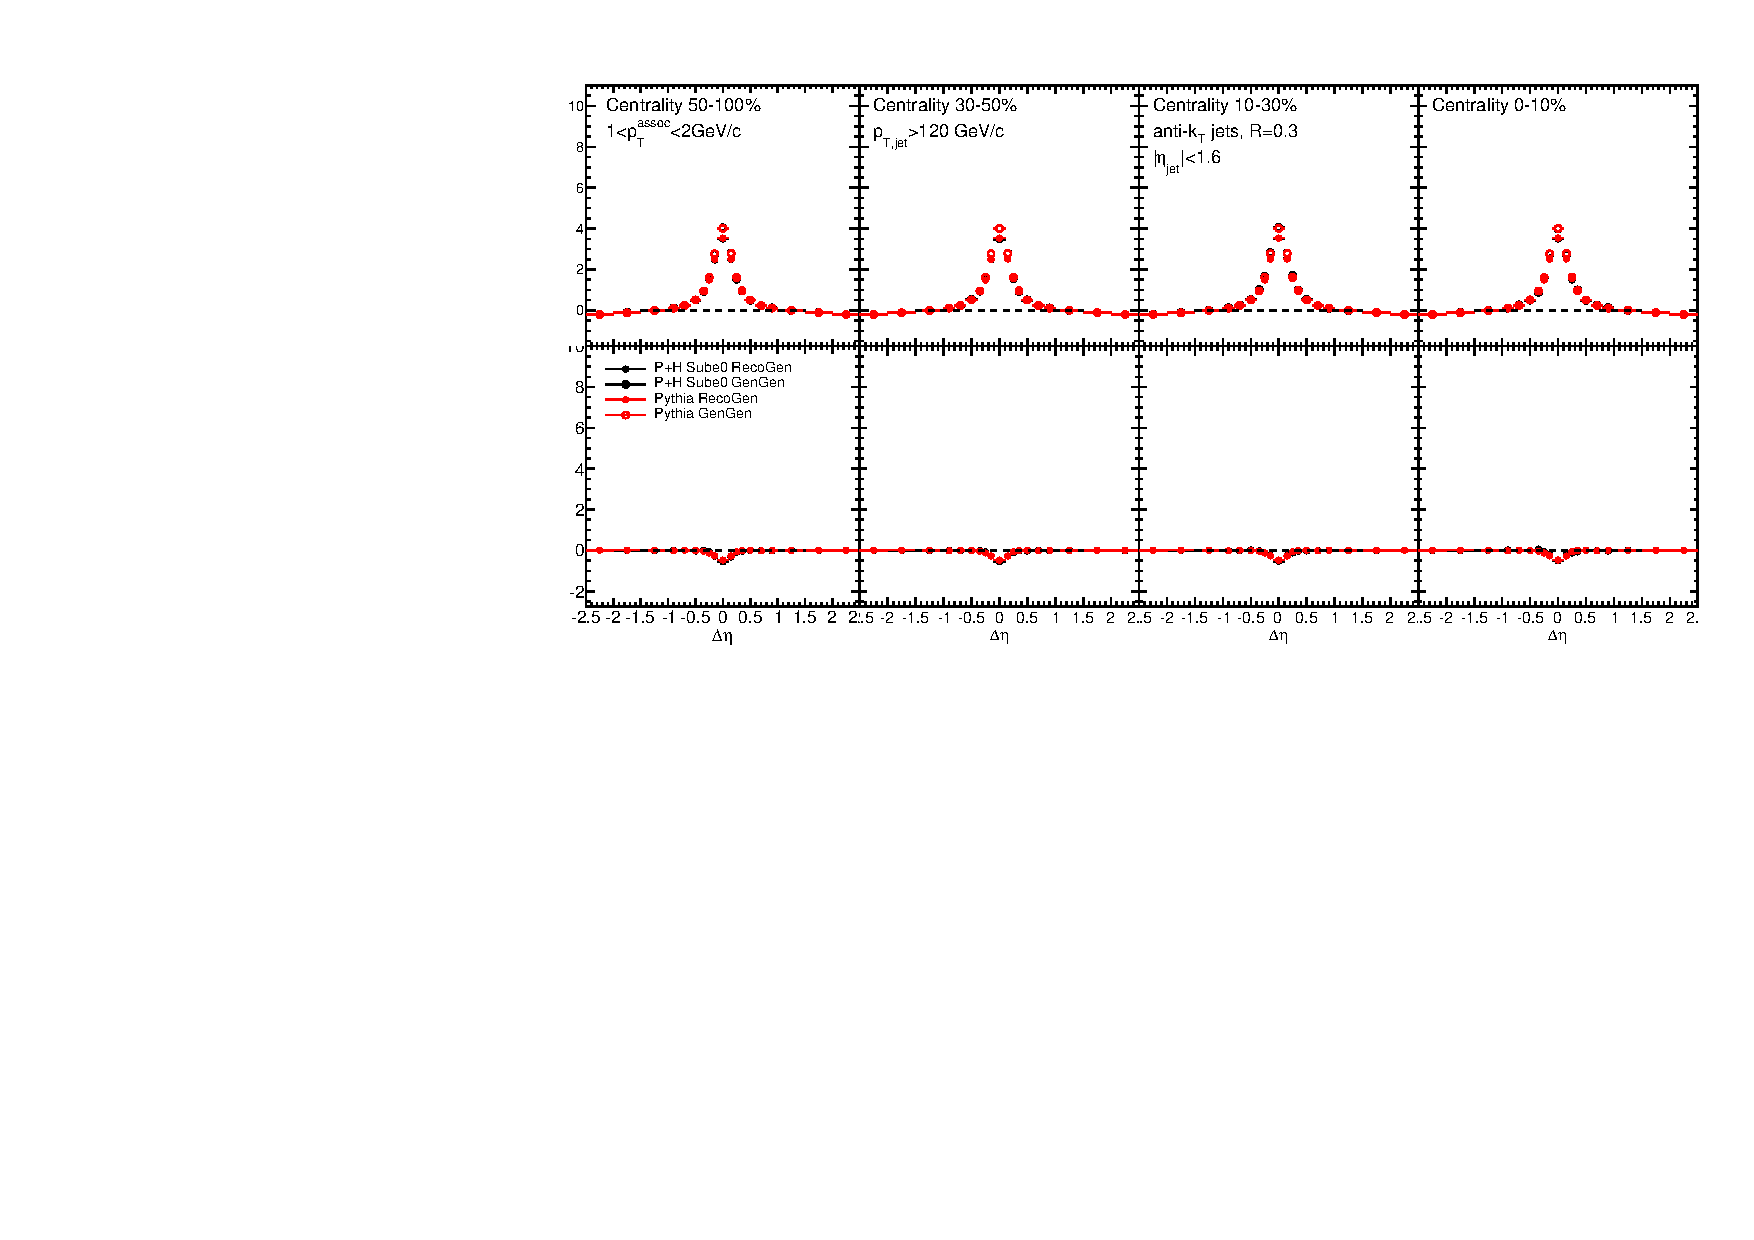
\includegraphics[width=0.99\textwidth]{figures/JFF_SpillOver/JFF_Residual_Corrections_Eta_Inclusive_TrkPt1_TrkPt2.pdf}
          \caption[Jet fragmentation function bias corrections for particles with $1<p_{\rm T}^{\rm trk}<2$ GeV]{$\Delta\eta$ jet fragmentation function bias corrections derived by comparing correlations between reconstructed vs. generated jets and generated {\sc pythia} events, with and without embedding into the {\sc hydjet} heavy ion environment, for particles $1<p_{\rm T}^{\rm trk}<2$ GeV.}
            \label{fig:jff_residual_inclusive_trkpt1_trkpt2}
            \end{center}
            \end{figure}
            
                      \begin{figure}[hbtp]
          \begin{center}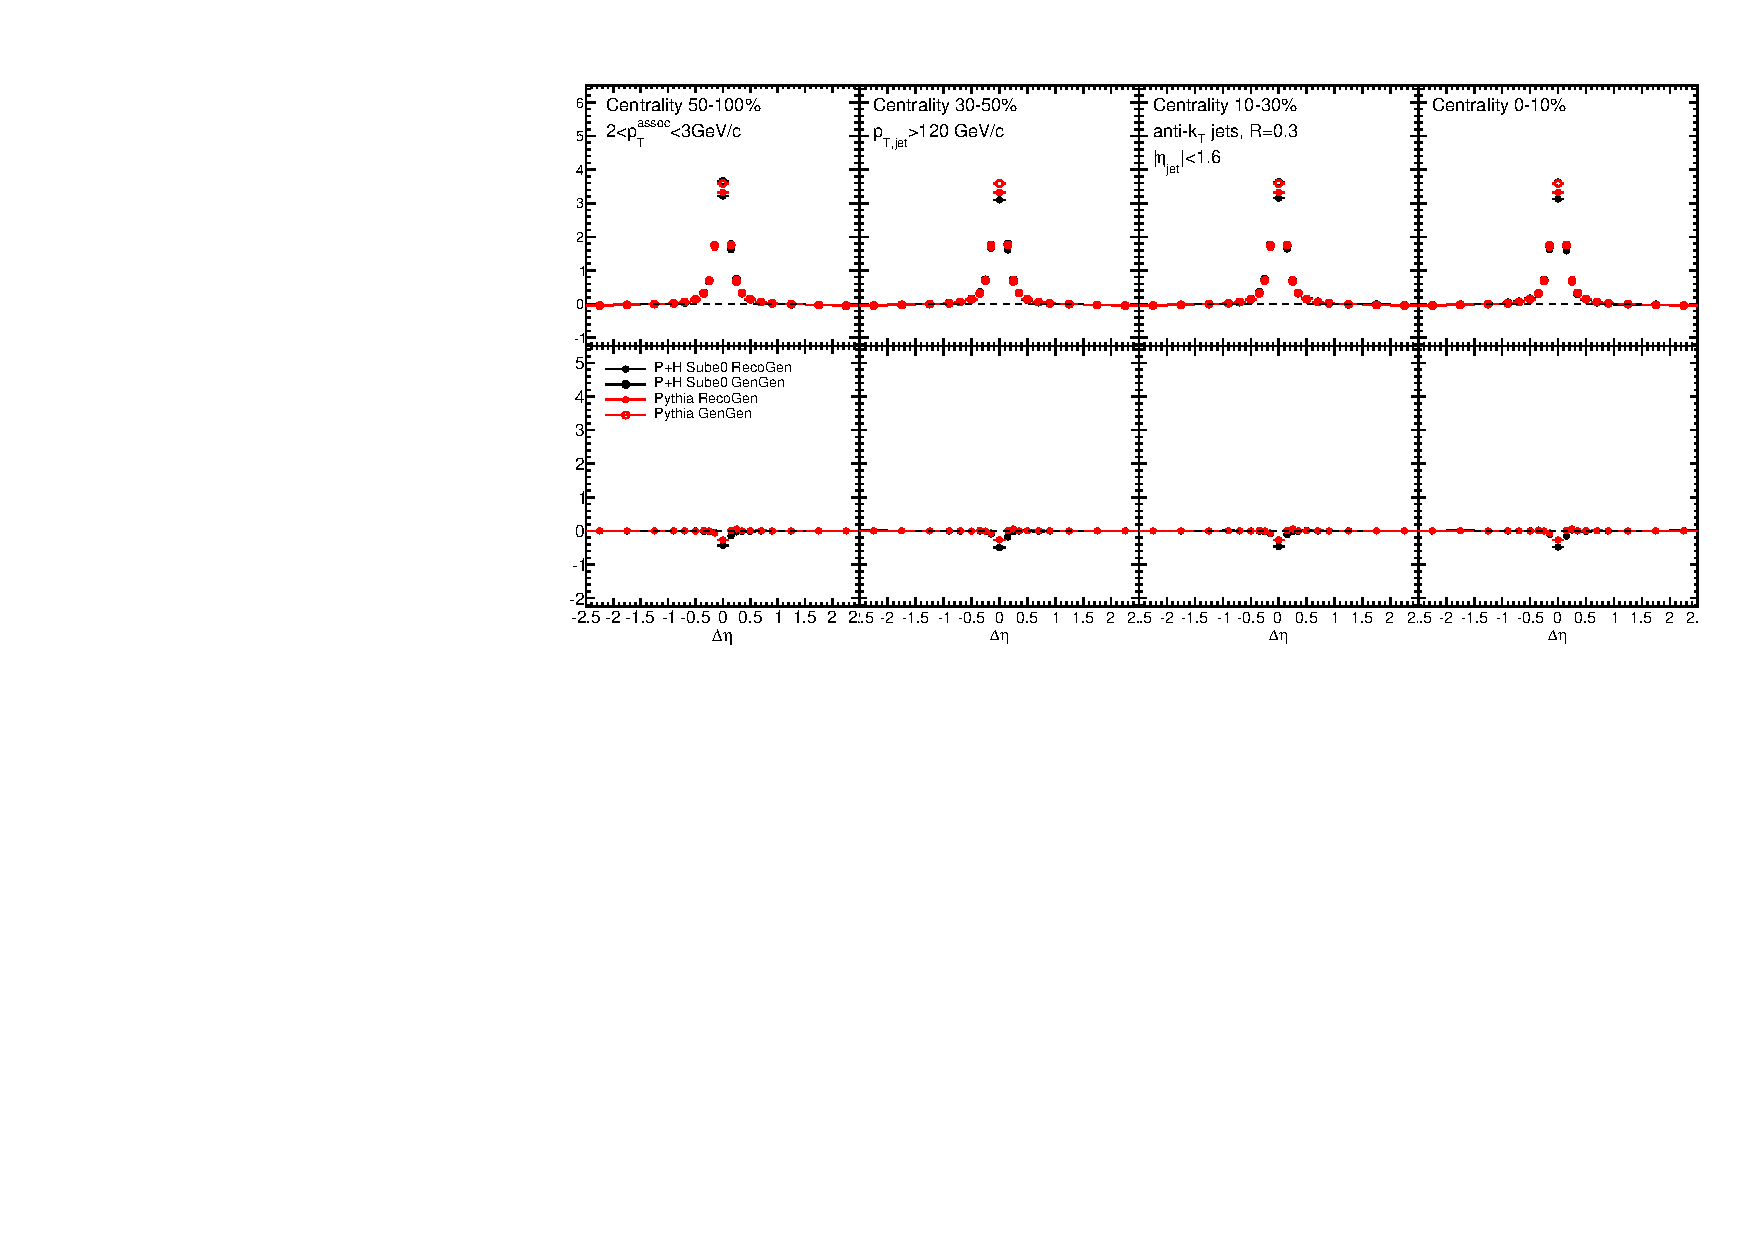
\includegraphics[width=0.99\textwidth]{figures/JFF_SpillOver/JFF_Residual_Corrections_Eta_Inclusive_TrkPt2_TrkPt3.pdf}
          \caption[Jet fragmentation function bias corrections for particles with $2<p_{\rm T}^{\rm trk}<3$ GeV]{$\Delta\eta$ jet fragmentation function bias corrections derived by comparing correlations between reconstructed vs. generated jets and generated {\sc pythia} events, with and without embedding into the {\sc hydjet} heavy ion environment, for particles $2<p_{\rm T}^{\rm trk}<3$ GeV.}
            \label{fig:jff_residual_inclusive_trkpt2_trkpt3}
            \end{center}
            \end{figure}
            
                      \begin{figure}[hbtp]
          \begin{center}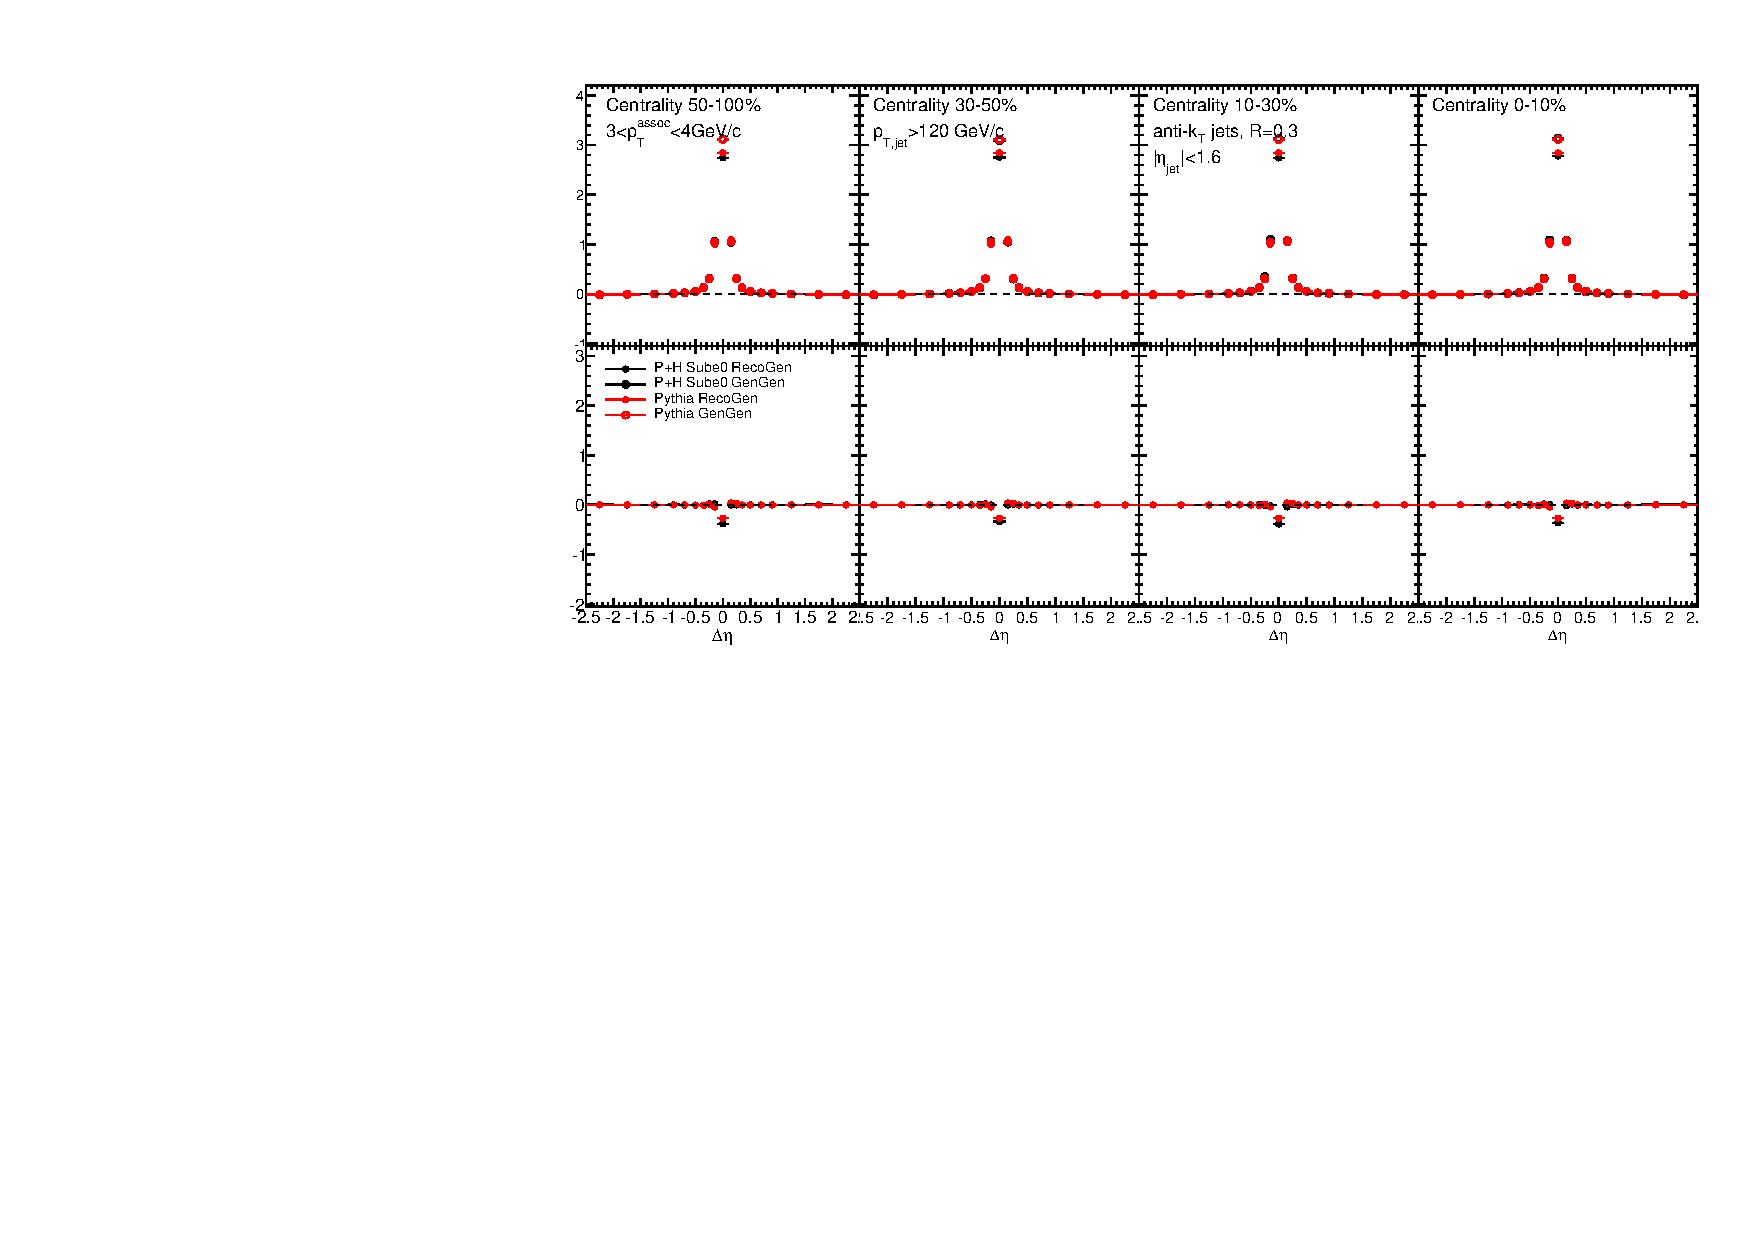
\includegraphics[width=0.99\textwidth]{figures/JFF_SpillOver/JFF_Residual_Corrections_Eta_Inclusive_TrkPt3_TrkPt4.pdf}
          \caption[Jet fragmentation function bias corrections for particles with $3<p_{\rm T}^{\rm trk}<4$ GeV]{$\Delta\eta$ jet fragmentation function bias corrections derived by comparing correlations between reconstructed vs. generated jets and generated {\sc pythia} events, with and without embedding into the {\sc hydjet} heavy ion environment, for particles $3<p_{\rm T}^{\rm trk}<4$ GeV.}
            \label{fig:jff_residual_inclusive_trkpt3_trkpt4}
            \end{center}
            \end{figure}
            
                      \begin{figure}[hbtp]
          \begin{center}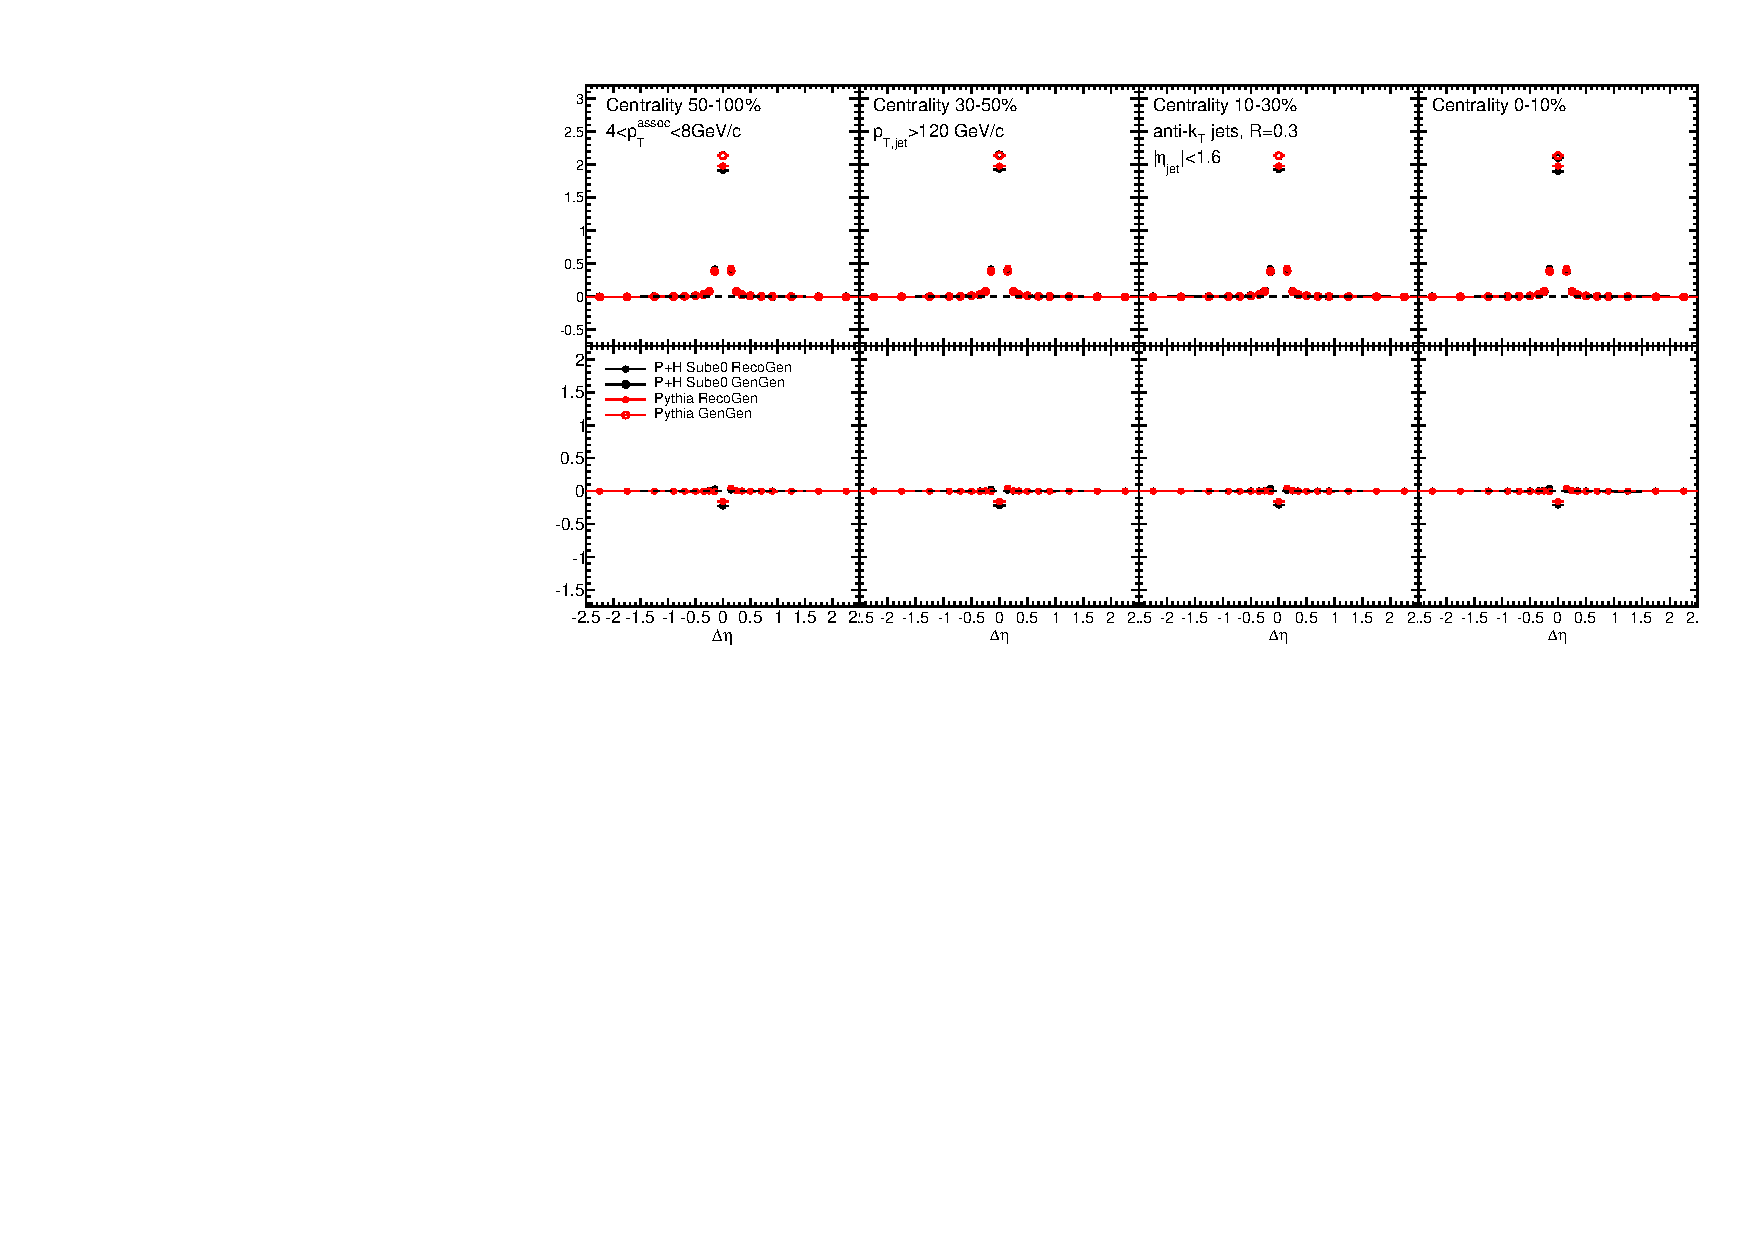
\includegraphics[width=0.99\textwidth]{figures/JFF_SpillOver/JFF_Residual_Corrections_Eta_Inclusive_TrkPt4_TrkPt8.pdf}
          \caption[Jet fragmentation function bias corrections for particles with $4<p_{\rm T}^{\rm trk}<8$ GeV]{$\Delta\eta$ jet fragmentation function bias corrections derived by comparing correlations between reconstructed vs. generated jets and generated {\sc pythia} events, with and without embedding into the {\sc hydjet} heavy ion environment, for particles $4<p_{\rm T}^{\rm trk}<8$ GeV.}
            \label{fig:jff_residual_inclusive_trkpt4_trkpt8}
            \end{center}
            \end{figure}
            
           \clearpage  
           
To assess the overall effect of these corrections, the integrated yield of these corrections is shown as a function of transverse momentum and centrality is shown for inclusive, leading, and subleading jets as a function of $p_{\rm T}^{\rm trk}$ in Fig.~\ref{fig:jff_residual_integrals_pT} and as a function of PbPb centrality in Fig.~\ref{fig:jff_residual_integrals_Cent}.  The correction magnitude shows little centrality dependence, and is very similar for pure {\sc pythia} simulation and {\sc pythia} embedded into {\sc hydjet}.  
            
                  \begin{figure}[h!]
                  \begin{center}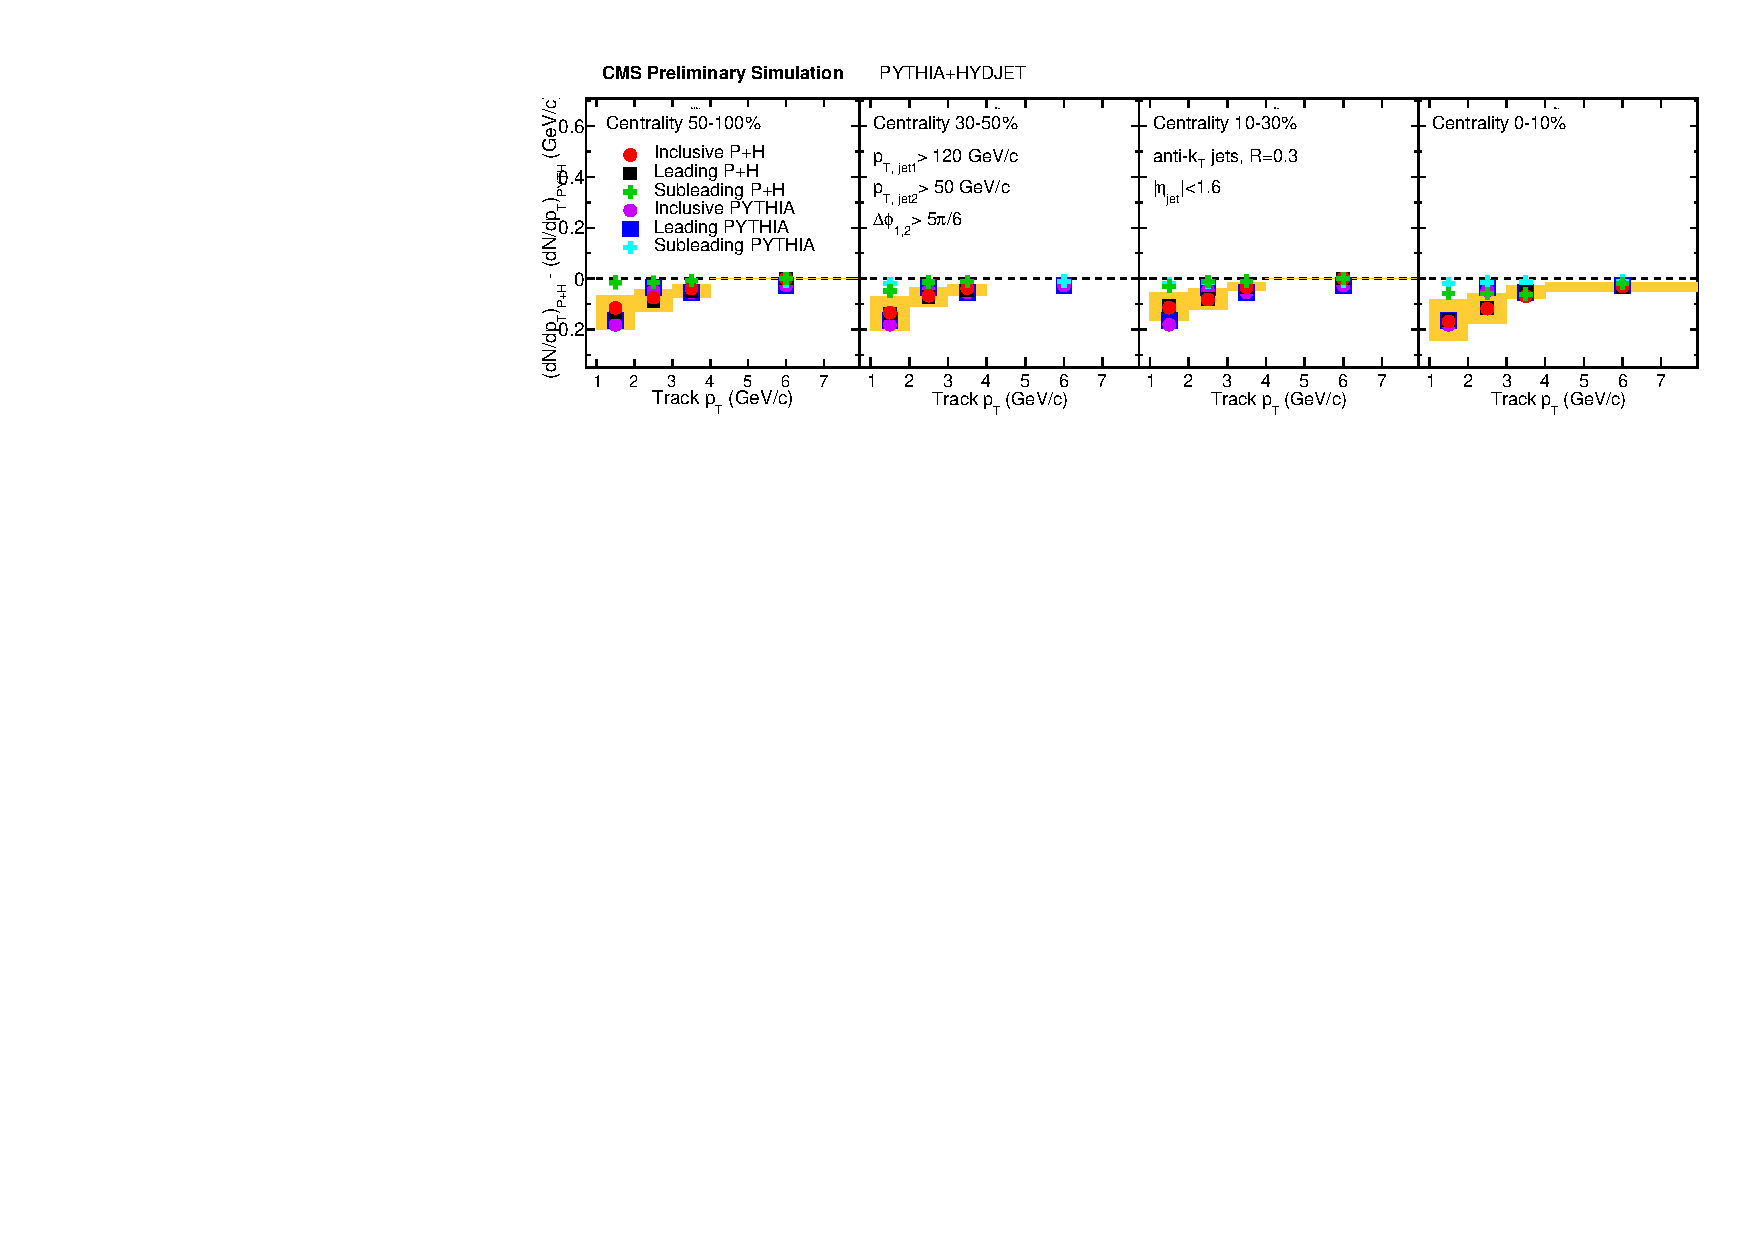
\includegraphics[width=0.99\textwidth]{figures/JFF_SpillOver/Integral_JFFResidual_pT.pdf}
                  \caption[Integrated yield attributed to jet fragmentation function bias as a function of $p_{\rm T}^{\rm trk}$]{Integrated yield attributed to jet fragmentation function bias in jet reconstruction for {\sc pythia} alone and embedded into {\sc hydjet}, shown as a function of $p_{\rm T}^{\rm trk}$ for each centrality class.}
                    \label{fig:jff_residual_integrals_pT}
                    \end{center}
                    \end{figure}

           
                  \begin{figure}[h!]
                  \begin{center}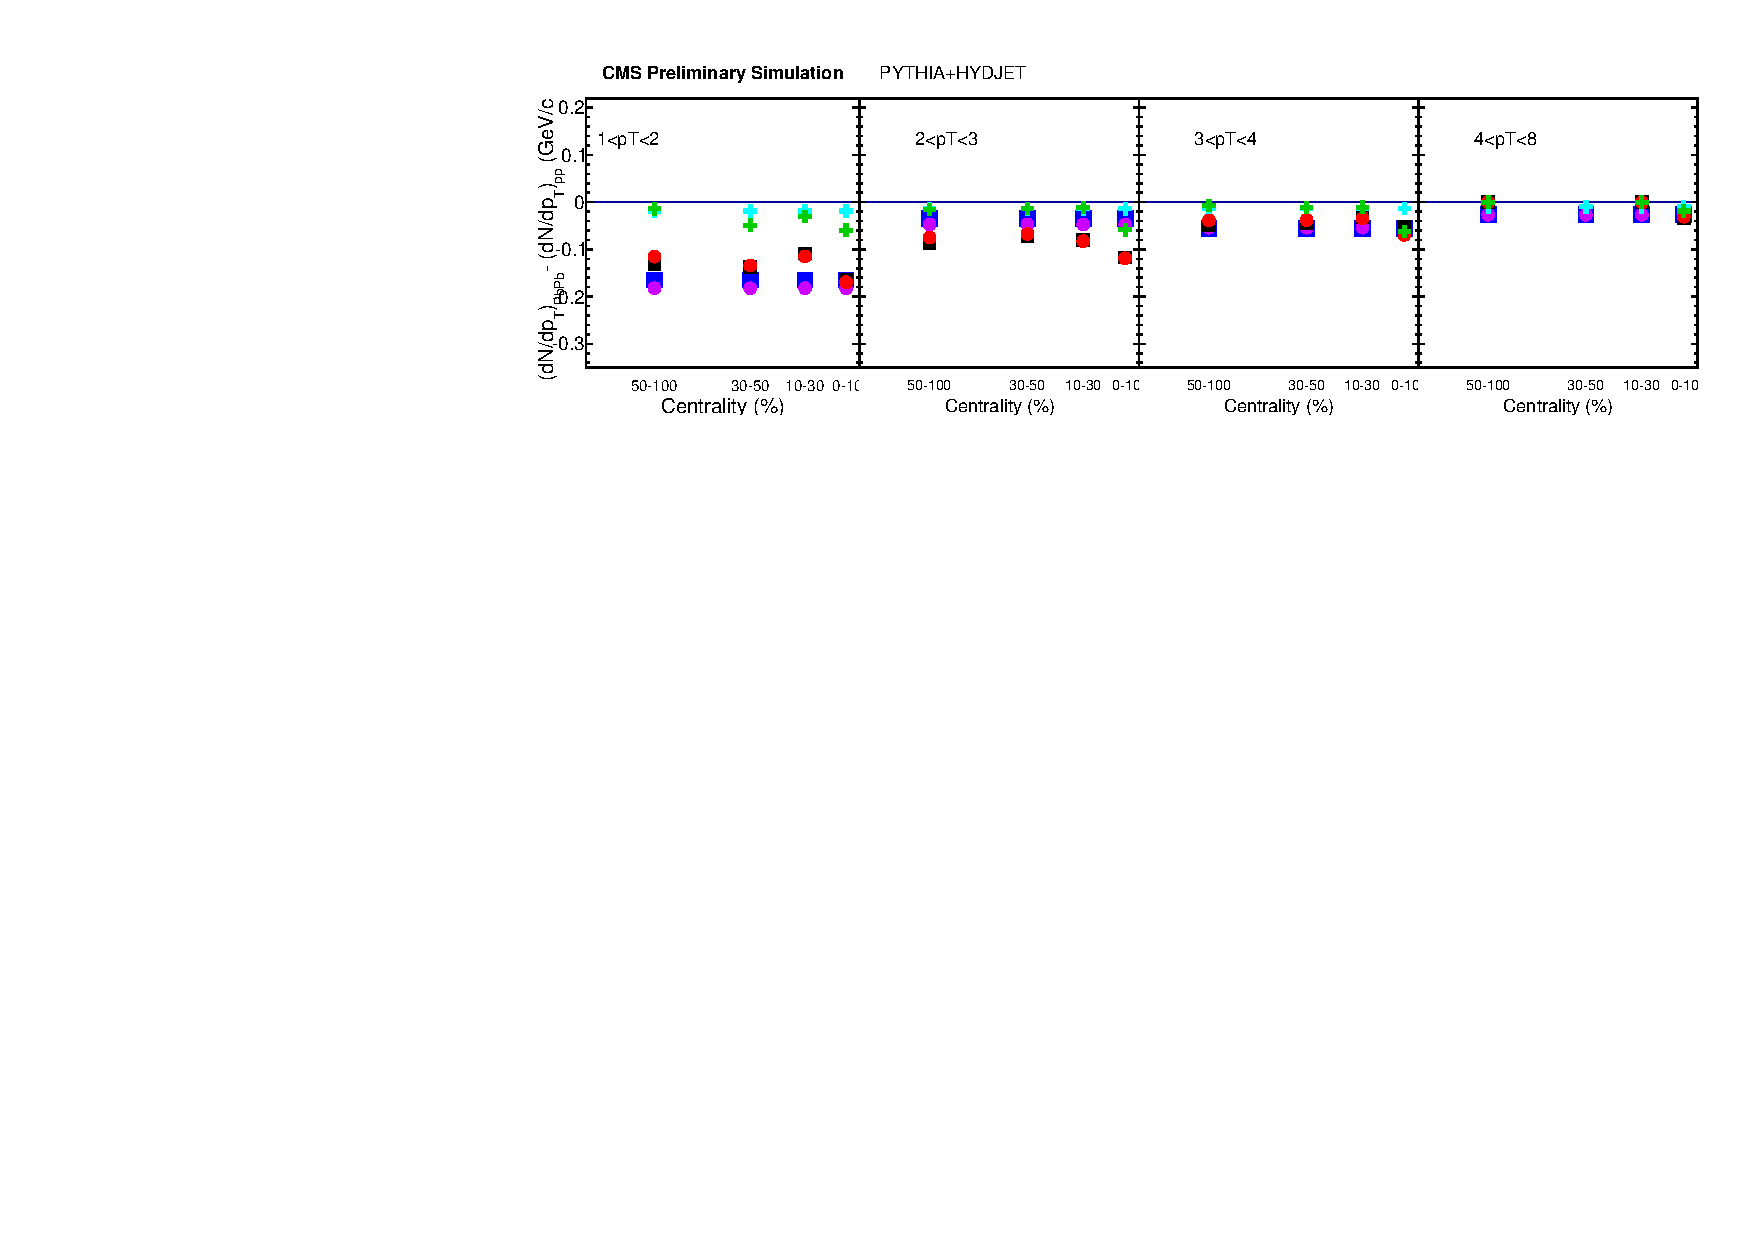
\includegraphics[width=0.99\textwidth]{figures/JFF_SpillOver/Integral_JFFResidual_Cent.pdf}
                  \caption[Integrated yield attributed to jet fragmentation function bias as a function of centrality]{Integrated yield attributed to jet fragmentation function bias in jet reconstruction for {\sc pythia} alone and embedded into {\sc hydjet}, shown as a function of centrality for each associate track $p_{\rm T}$ range.}
                    \label{fig:jff_residual_integrals_Cent}
                    \end{center}
                    \end{figure}
                    
\clearpage




\subsection{Background fluctuation bias correction}

In central PbPb collisions background levels are very high, and naturally fluctuate throughout the event.  As discussed in Section~\ref{sec:Jets}, the process of jet reconstruction in PbPb collisions includes background subtraction that accounts for the general distirbution of energy in the event.  However, small, local variations in background levels remain (on the order of 5 GeV within a radius of R = 0.3).  These are reconstructed into the jet, raising or lowering the measured jet energy depending on whether the jet sits on an upward or a downward fluctuation in the background.  As a result, jets with ``true'' $p_{\rm T}$ slightly below the 120 GeV selection threshold that sit on upward background fluctuations will be included in the sample, while jets sit on downward will be excluded.  Because the jet spectrum is steeply falling, it is much more common for a lower-$p_{\rm T}$ jet (on an upward fluctuation) to be included in the sample than for a higher-$p_{\rm T}$ jet to be excluded.  This results in the systematic inclusion of tracks from background fluctuations in the peak of tracks observed about the jet axis, resulting in a contribution to the initially measured jet peak that must be accurately quantified and subtracted.  

To estimate and subtract the contribution to the excess yield due to background fluctuation bias in jet reconstruction  to the measured excess yield, we perform simulations in {\sc pythia+hydjet} samples with reconstructed jets (but generated tracks, as the tracking efficiency uncertainty is analyzed separately), and construct correlations excluding particles generated with the embedded {\sc pythia} hard-scattering process.  As the {\sc pythia+hydjet} simulation does not include interactions between the {\sc pythia} hard process and the medium, this procedure by construction isolates the contribution to the jet peak that is attributable to the background fluctuation bias. The resulting corrections are illustrated in Fig.~\ref{fig:reco_reco_closure_deta_inc} -  Fig.~\ref{fig:reco_reco_closure_inc4} for inclusive jets at 2.76 TeV.  These correlations show a diminishing effect with increasing particle transverse momentum.  We subtract the gaussian fit to these correlations bin-by-bin from the data results, and also assign the half its magnitude as systematic uncertainty to the final measurements.  To assess the overall effect of these corrections, the integrated yield of these corrections is shown in Fig.~\ref{fig:closure_integrals_pT} as a function of transverse momentum and centrality is shown for inclusive, leading, and subleading jets at 2.76 TeV. 


      \begin{figure}[hbtp]
      \begin{center}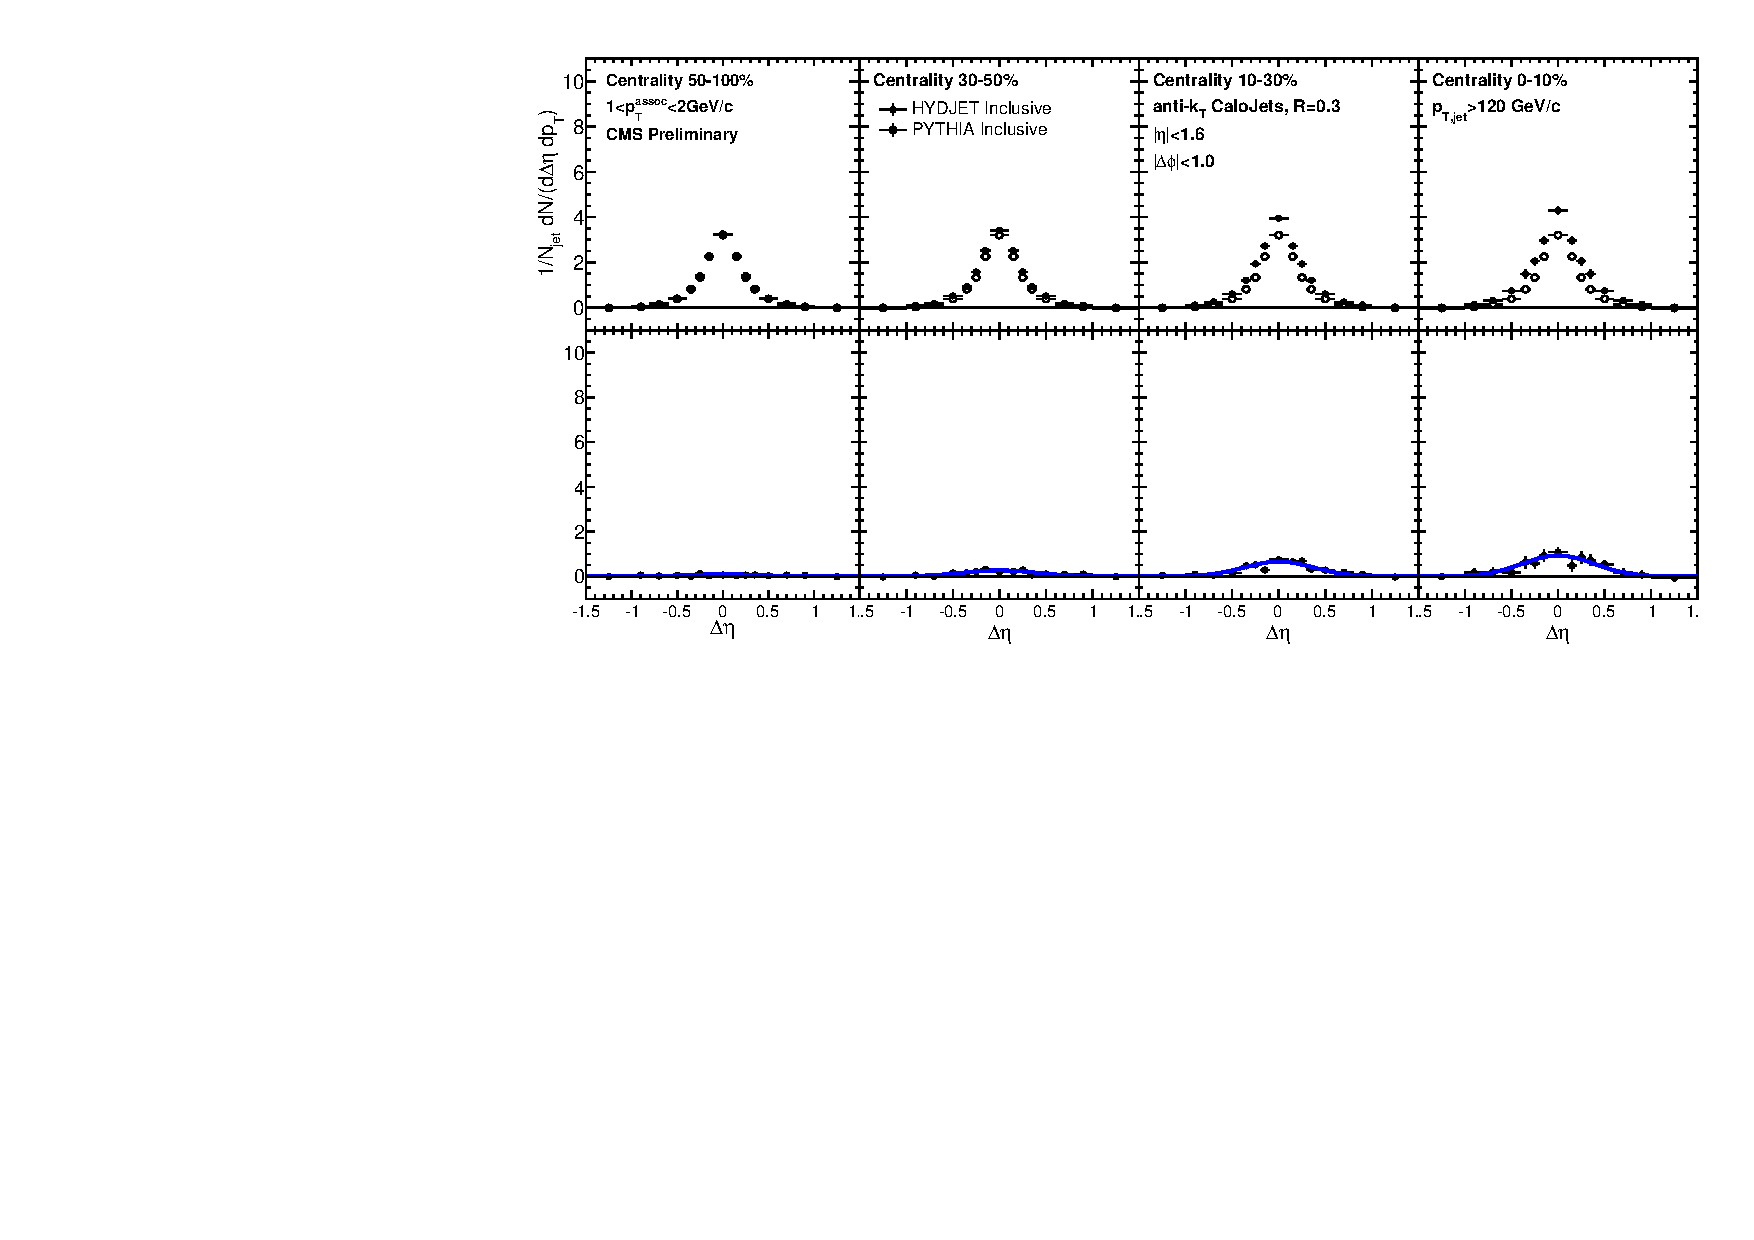
\includegraphics[width=0.99\textwidth]{figures/JFF_SpillOver/AN_Closures_Eta_InclusiveTrkPt1_TrkPt2.pdf}
      \caption[Background fluctuation bias corrections for particles with $1<p_{\rm T}^{\rm trk}<2$ GeV]{$\Delta\eta$ background fluctuation bias correction for inclusive jets derived by constructing correlations in {\sc pythia+hydjet} between reconstructed jets and only those tracks simulated as part of the heavy ion underlying event rather than the embedded {\sc pythia} hard process, for particles $1<p_{\rm T}^{\rm trk}<2$ GeV}
        \label{fig:reco_reco_closure_deta_inc}
        \end{center}
        \end{figure}



   \begin{figure}[hbtp]
              \begin{center}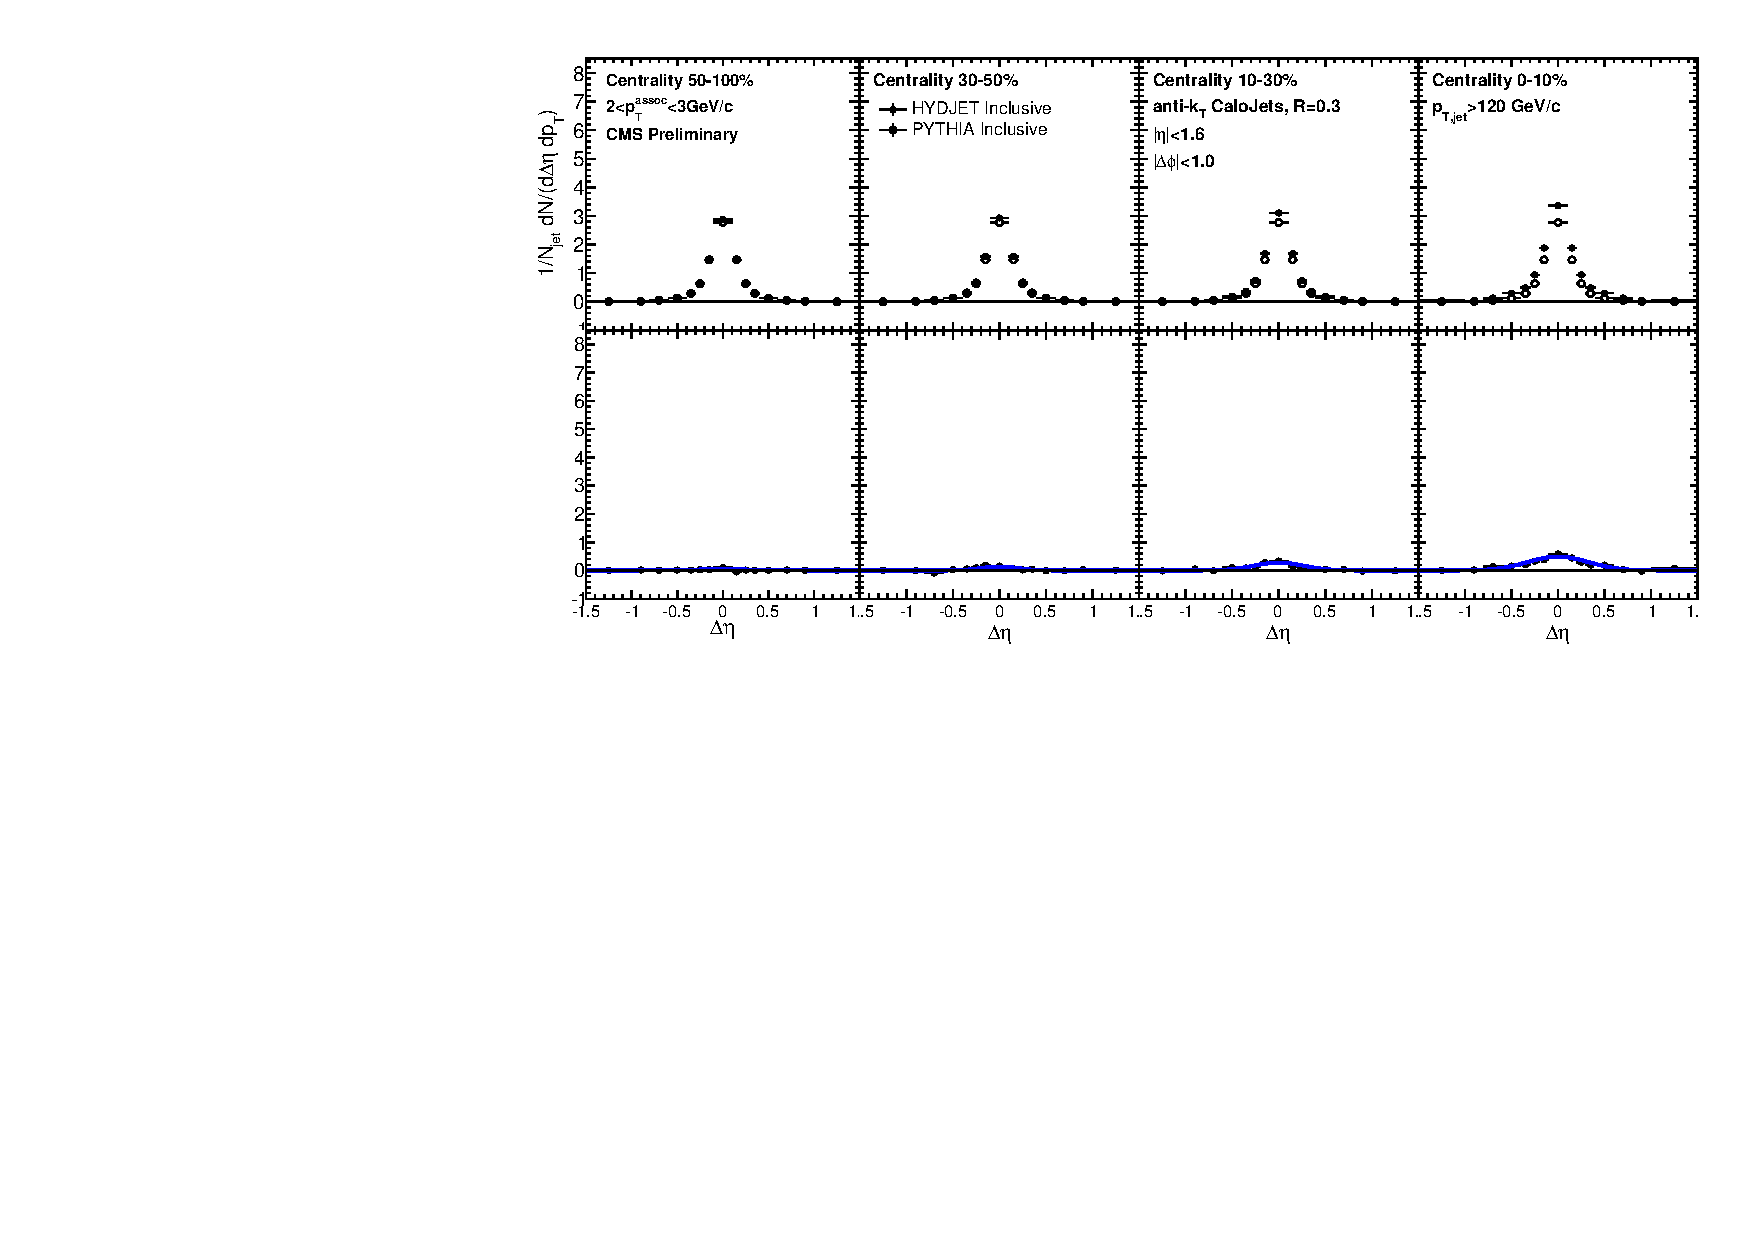
\includegraphics[width=0.99\textwidth]{figures/JFF_SpillOver/AN_Closures_Eta_InclusiveTrkPt2_TrkPt3.pdf}
             \caption[Background fluctuation bias corrections for particles with $2<p_{\rm T}^{\rm trk}<3$ GeV]{$\Delta\eta$ background fluctuation bias correction for inclusive jets derived by constructing correlations in {\sc pythia+hydjet} between reconstructed jets and only those tracks simulated as part of the heavy ion underlying event rather than the embedded {\sc pythia} hard process, for particles $2<p_{\rm T}^{\rm trk}<3$ GeV}
                \label{fig:reco_reco_closure_inc2}
                \end{center}
                \end{figure}

                \begin{figure}[hbtp] 
                \begin{center}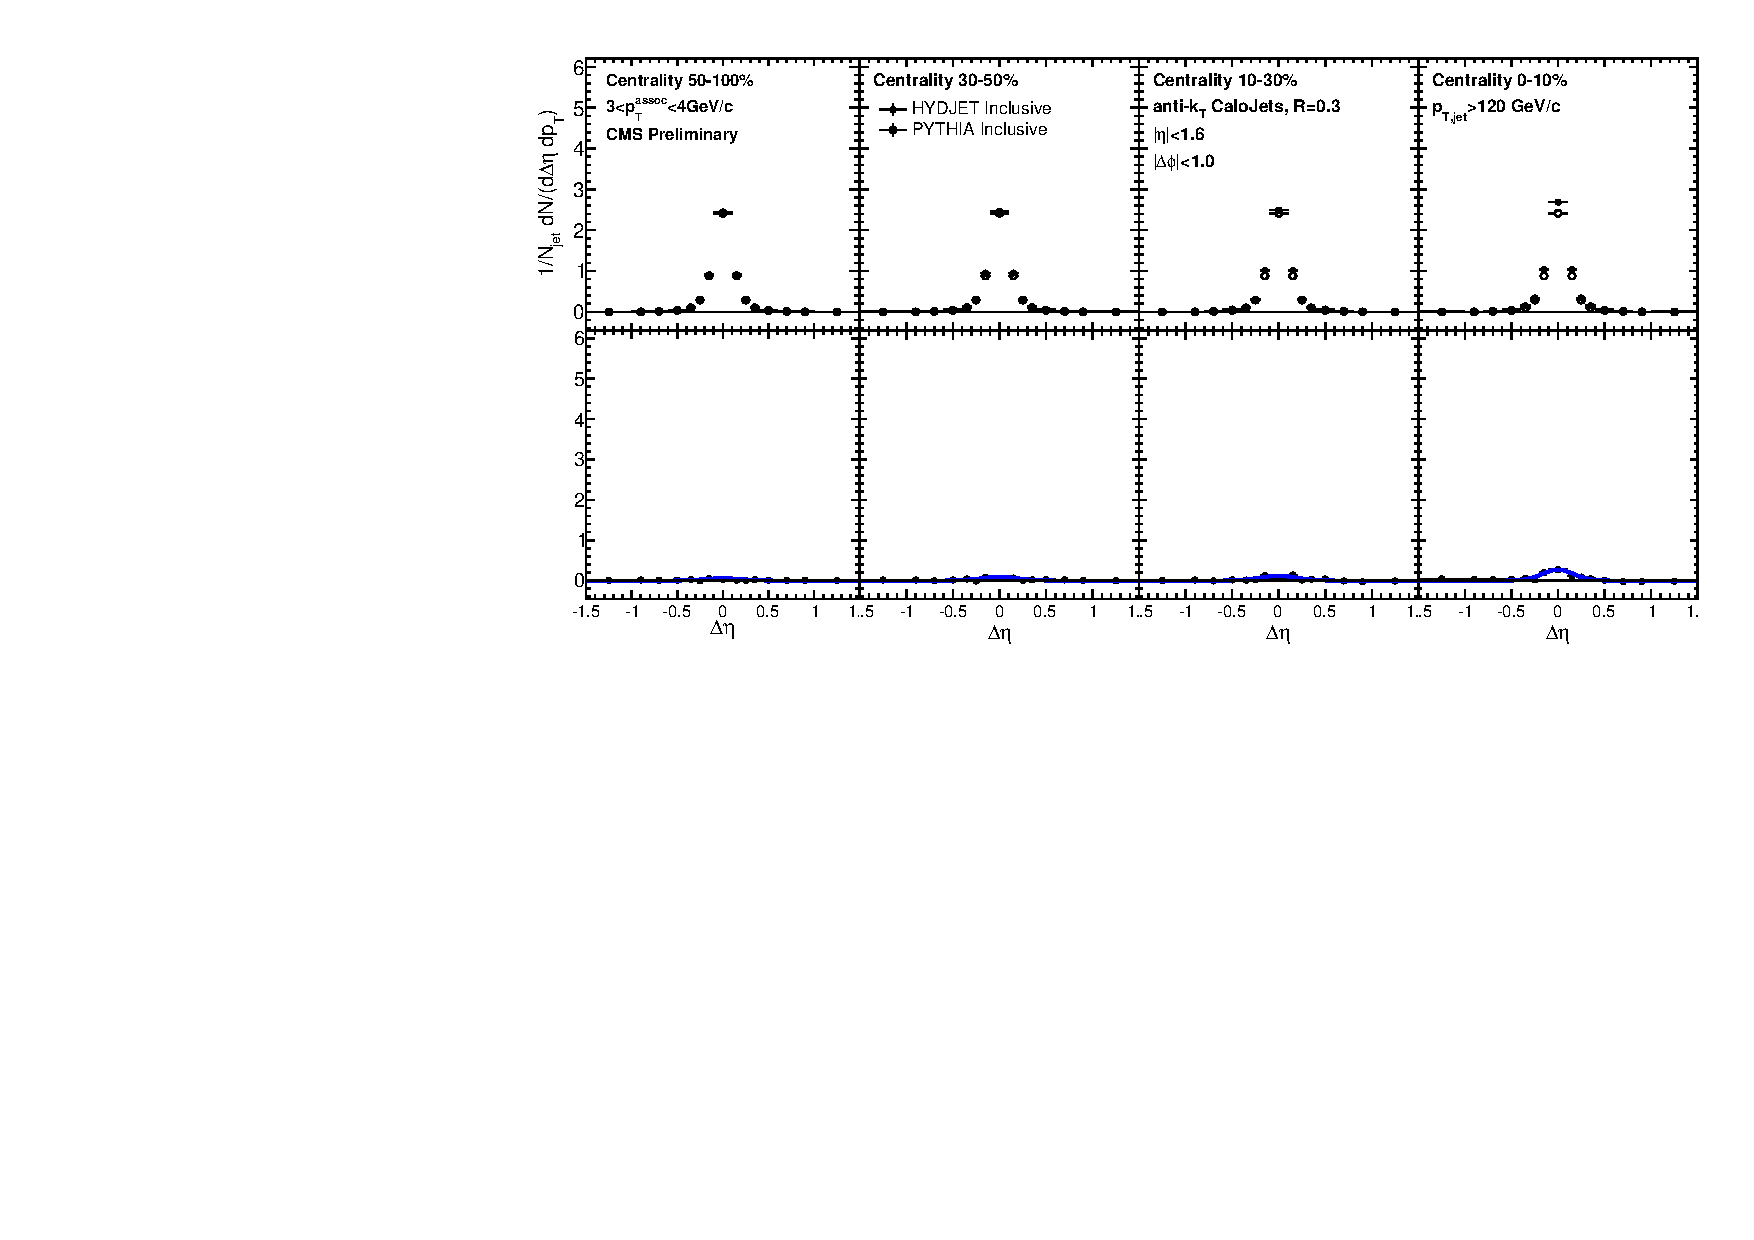
\includegraphics[width=0.99\textwidth]{figures/JFF_SpillOver/AN_Closures_Eta_InclusiveTrkPt3_TrkPt4.pdf}
               \caption[Background fluctuation bias corrections for particles with $3<p_{\rm T}^{\rm trk}<4$ GeV]{$\Delta\eta$ background fluctuation bias correction for inclusive jets derived by constructing correlations in {\sc pythia+hydjet} between reconstructed jets and only those tracks simulated as part of the heavy ion underlying event rather than the embedded {\sc pythia} hard process, for particles $3<p_{\rm T}^{\rm trk}<4$ GeV}

                  \label{fig:reco_reco_closure_inc3}
                  \end{center}
                  \end{figure}


                  \begin{figure}[hbtp]
                  \begin{center}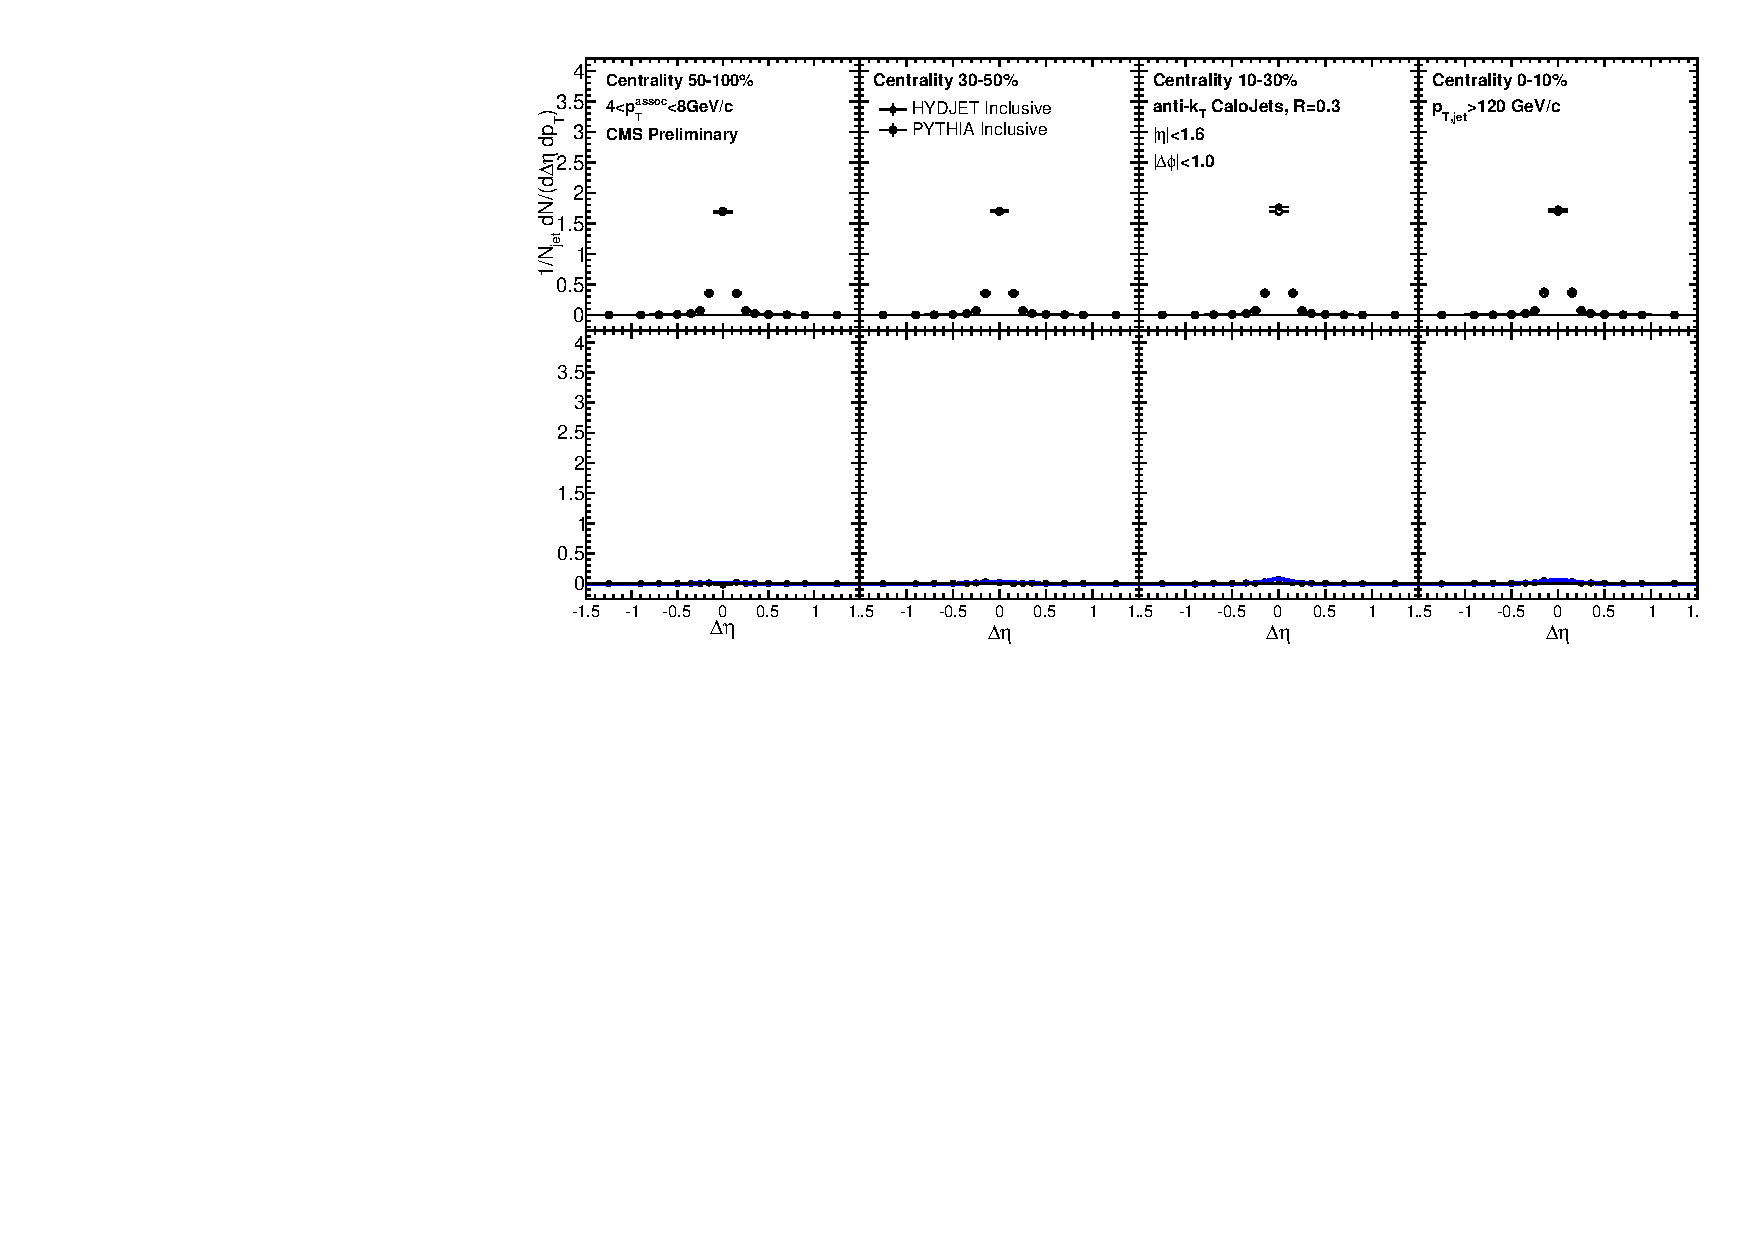
\includegraphics[width=0.99\textwidth]{figures/JFF_SpillOver/AN_Closures_Eta_InclusiveTrkPt4_TrkPt8.pdf}
                 \caption[Background fluctuation bias corrections for particles with $4<p_{\rm T}^{\rm trk}<8$ GeV]{$\Delta\eta$ background fluctuation bias correction for inclusive jets derived by constructing correlations in {\sc pythia+hydjet} between reconstructed jets and only those tracks simulated as part of the heavy ion underlying event rather than the embedded {\sc pythia} hard process, for particles $4<p_{\rm T}^{\rm trk}<8$ GeV}
                    \label{fig:reco_reco_closure_inc4}
                    \end{center}
                    \end{figure}

       
                  \begin{figure}[h!]
                  \begin{center}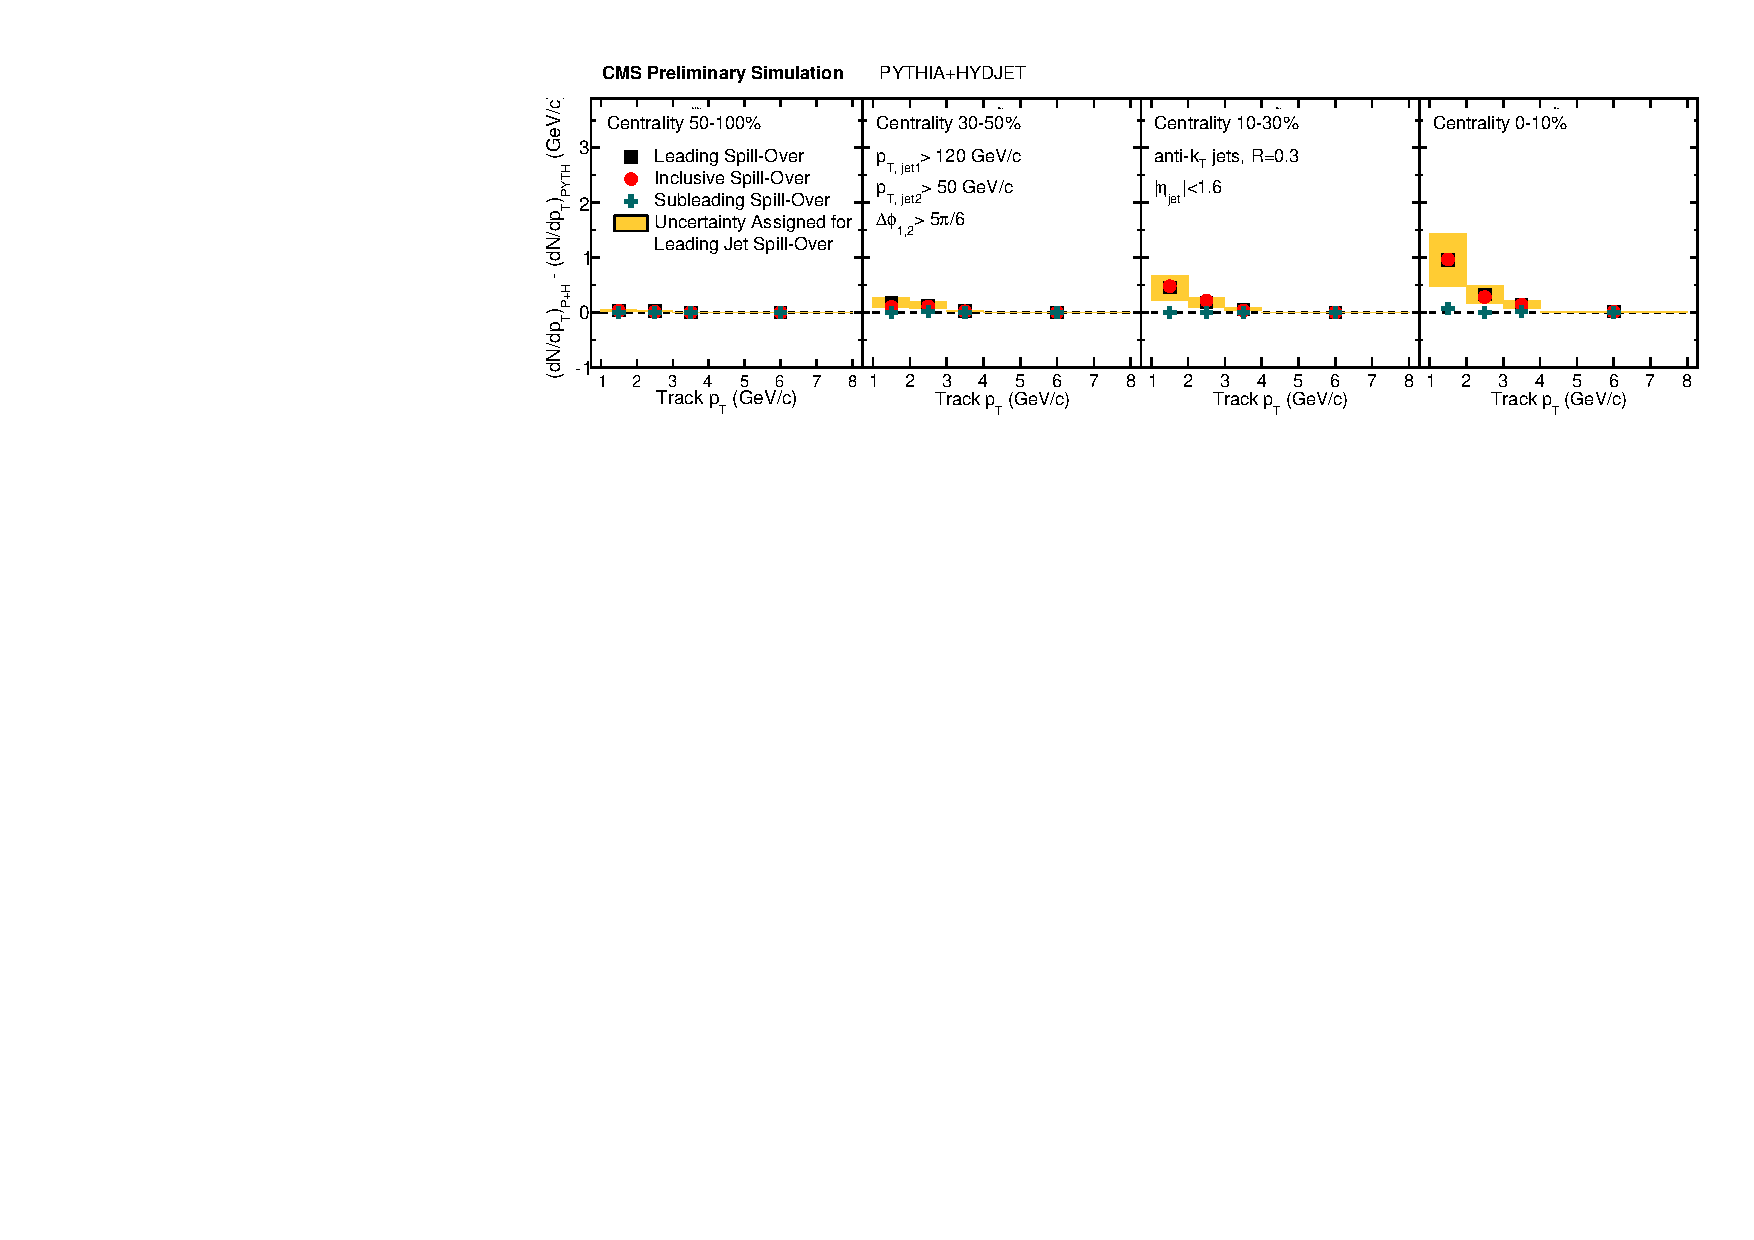
\includegraphics[width=0.99\textwidth]{figures/JFF_SpillOver/Integral_Closure_pT_Leading.pdf}
                  \caption[Integrated yield attributed to background fluctuation bias as a function of $p_{\rm T}^{\rm trk}$]{Integrated yield attributed to background fluctuation bias in the selection of inclusive and leading jets, shown as a function of associate track $p_{\rm T}$ for each centrality class.}
                    \label{fig:closure_integrals_pT}
                    \end{center}
                    \end{figure}
                    

Considering that the background fluctuation bias effect in many ways mimics the jet peak signal, it is particularly important to validate this correction and confirm both that its origin is well-understood and that the {\sc hydjet} simulation used to derive it reproduces the background fluctuations in data closely enough to accurately obtain corrections.  To check this, we extract a direct estimate of the effect from data using a ``pseudo-embedding'' of pp jets into a minimum bias PbPb data sample.  The goal of this study is to verify that we recover a similar magnitude of excess yield as we attribute based on our more detailed {\sc pythia+hydjet} simulations.  Here we approximate the effect by adding the total transverse momentum in a circle of radius  $R = 0.3$ around all jets with $p_{\rm T} > 90$ GeV, and considering the total deviation up or down of this $(\Sigma p_{\rm T})_{\rm cone}$ from the average total transverse momentum $< (\Sigma p_{\rm T})_{\rm cone}>$.  First, we may directly compare the average $p_{\rm T}$ and fluctuations in $p_{\rm T}$ in these random cones between data and Monte Carlo.  We find that our Monte Carlo approximately reproduces the data:  in data $< (\Sigma p_{\rm T})_{\rm cone, data}> = 10.0$ GeV, with $\sigma((\Sigma p_{\rm T})_{\rm cone, data}) = 4.9$ GeV, while in Monte Carlo $< (\Sigma p_{\rm T})_{\rm cone, MC}> = 11.9$ GeV, with $\sigma((\Sigma p_{\rm T})_{\rm cone, data}) = 5.6$ GeV. 

We then use these random cones to adjust jet energy and re-select jets:  we add the deviation up or down of this $(\Sigma p_{\rm T})_{\rm cone}$ to each embedded pp jets with this adjusted $p_{\rm T}$.  We then fill $\Delta\eta - \Delta\phi$ correlations to all jets that pass our nominal $p_{\rm T} > 120$ GeV jet selection cut.  We apply this technique to both our {\sc pythia+hydjet} sample and a minimum-bias PbPb data sample to measure the charged particle yield associated with the embedded jet axis as a result of the jet fluctuation bias.  As Fig.~\ref{fig:data_spill_int}--\ref{fig:data_spill_bins} show, this data pseudo-embedding recovers the same magnitude of excess yield due to background fluctuation bias as our nominal Monte Carlo studies, but artificially confines this effect to a $R = 0.3$ cone by construction, due to the artificially simple jet reconstruction procedure.  This gives confidence that the origin and magnitude of the effect are well-understood.

\begin{figure}[h!]
\begin{center}
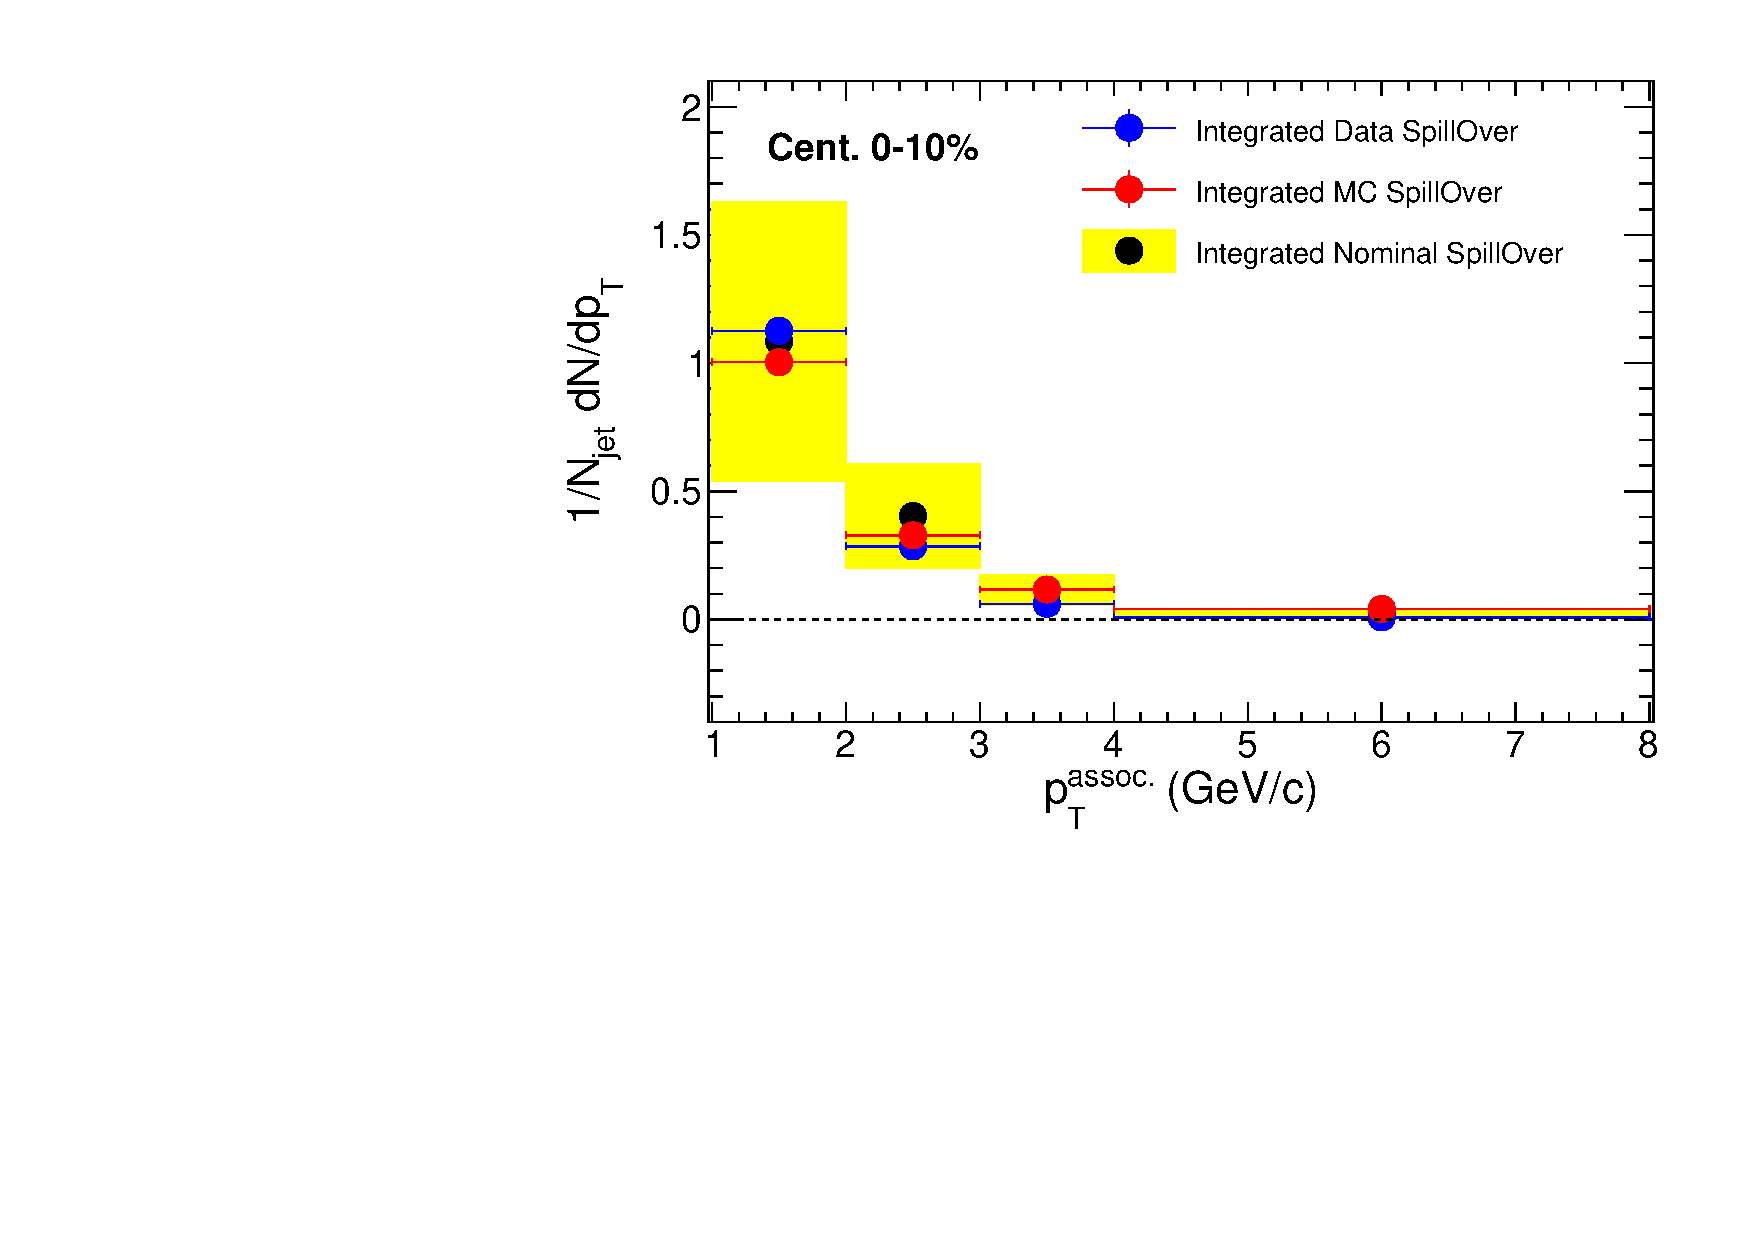
\includegraphics[width=0.49\textwidth]{figures/JFF_SpillOver/Data_Closure_Integrals.pdf}

\caption[Data-driven check of integrated yields attributed to background fluctuation bias]{Total integrated magnitude of background fluctuation bias as simulated with pp jets embedded in Minimum Bias events (blue points) compared to the effect as simulated with {\sc pythia}  jets into minimum bias {\sc hydjet} and to nominal corrections obtained with full {\sc pythia+hydjet} simulation. Nominal systematic errors of +/- 50\% as assigned in this analysis are shown as yellow systematic error bars on nominal (full MC simulation) points.}
\label{fig:data_spill_int}
\end{center}
\end{figure}


\begin{figure}[h!]
\begin{center}
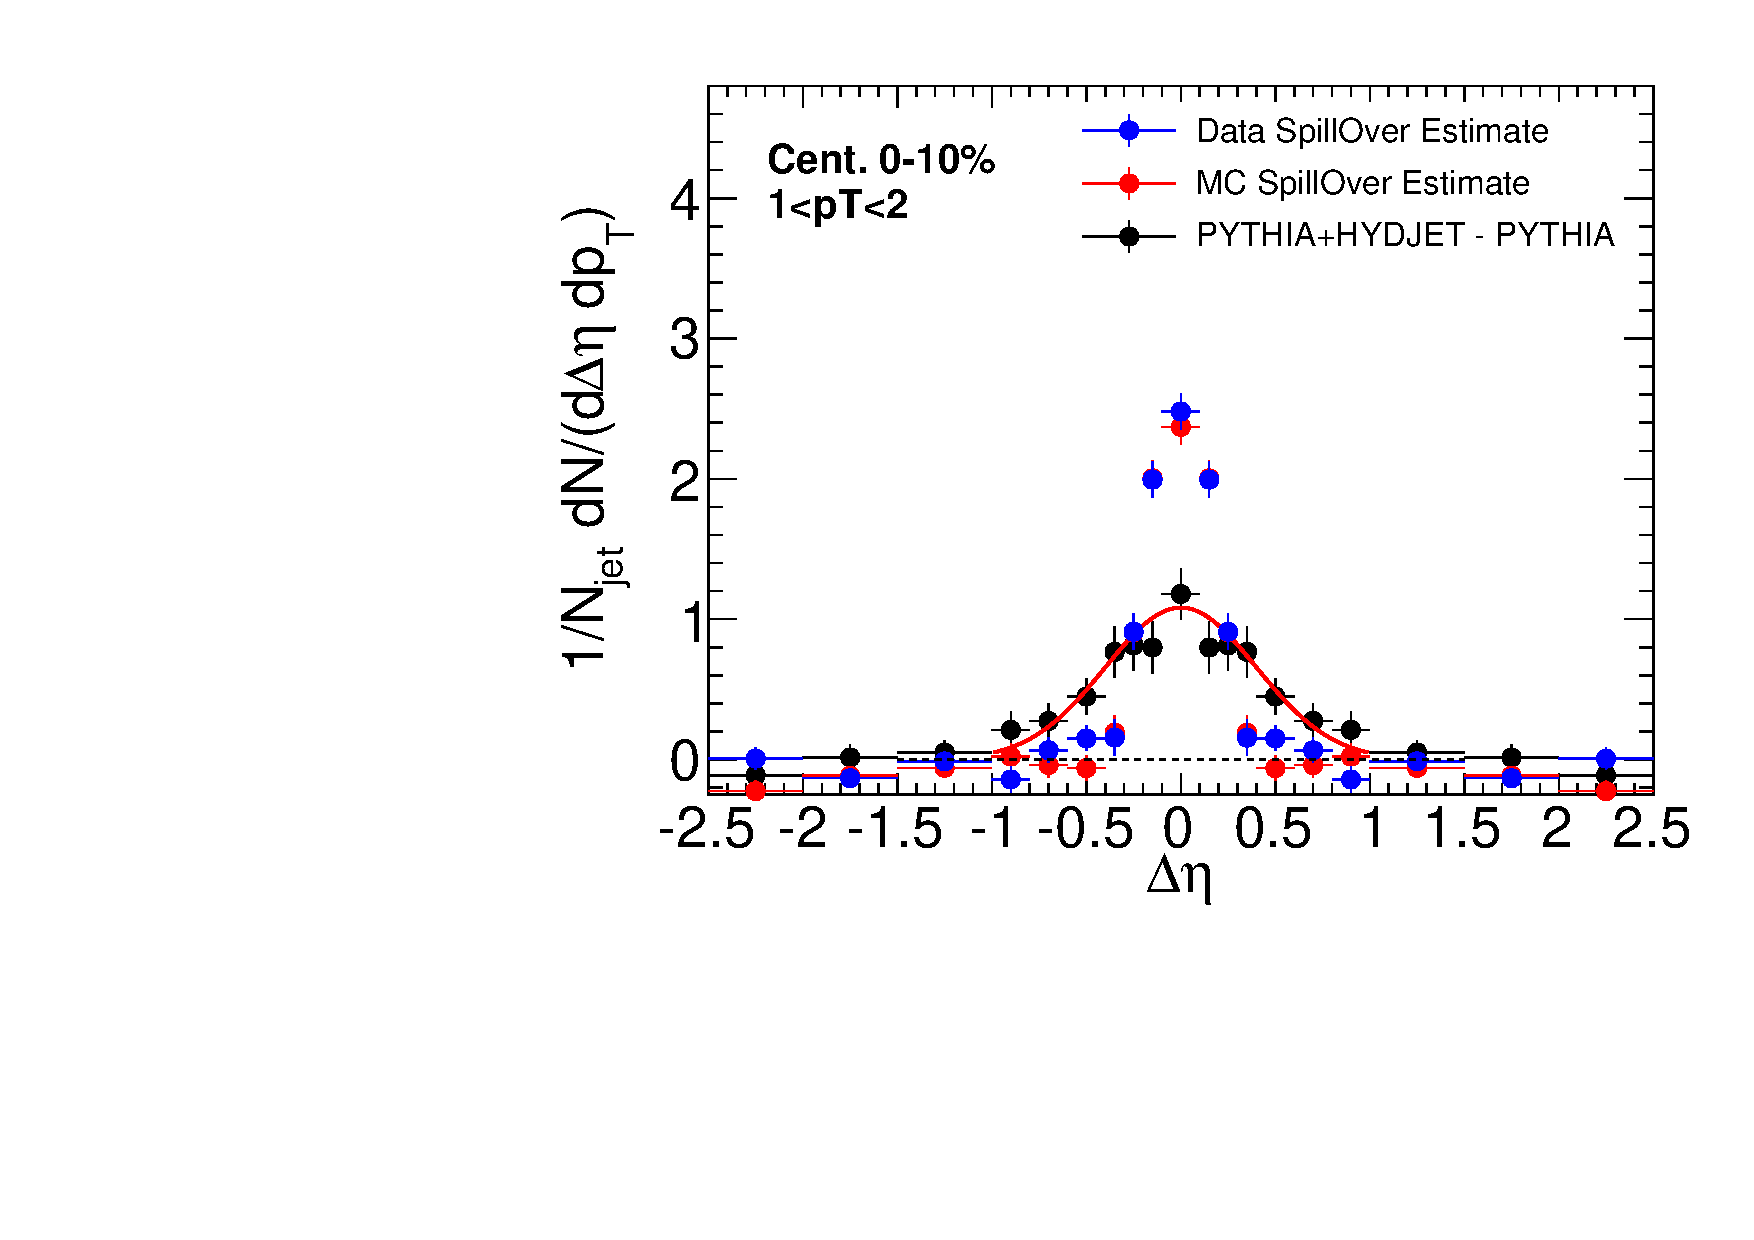
\includegraphics[width=0.49\textwidth]{figures/JFF_SpillOver/Data_Closures_TrkPt1_TrkPt2.pdf}
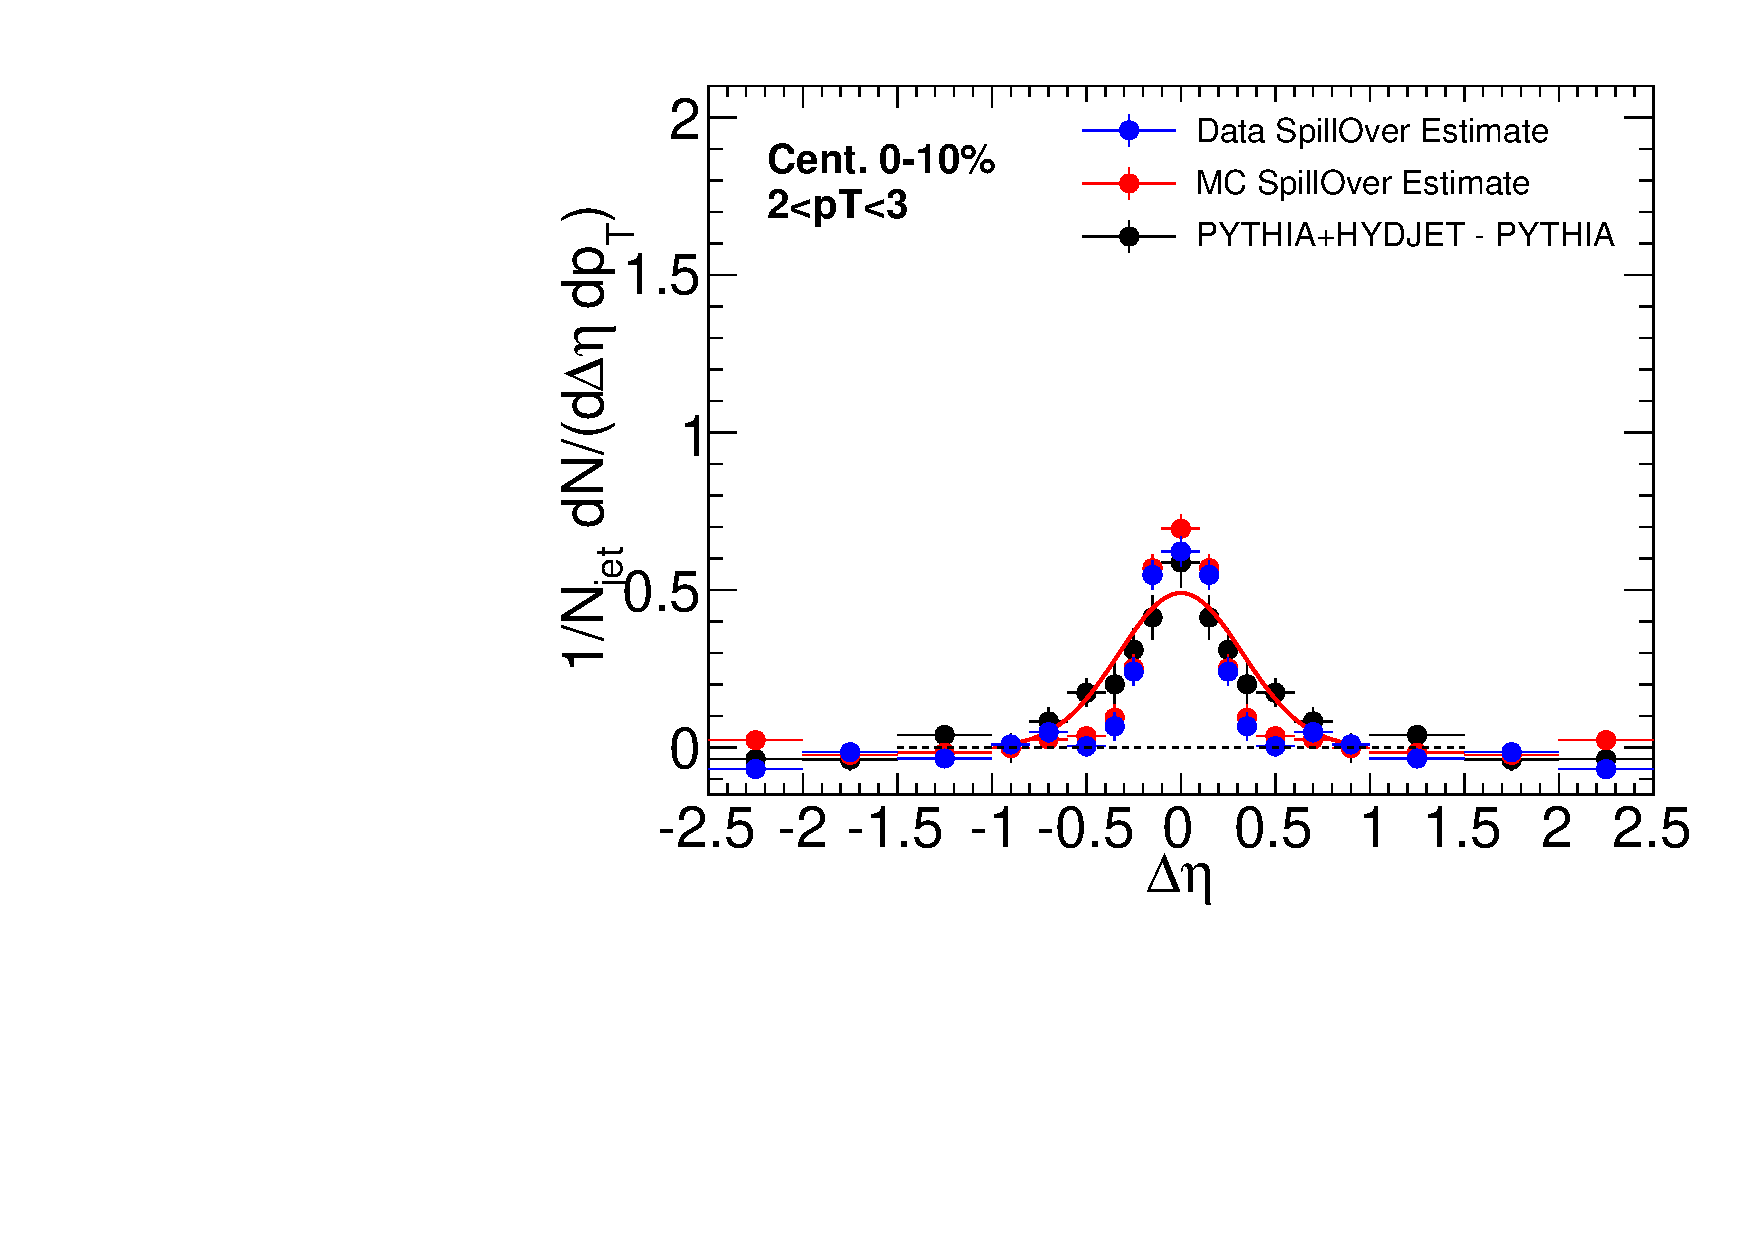
\includegraphics[width=0.49\textwidth]{figures/JFF_SpillOver/Data_Closures_TrkPt2_TrkPt3.pdf}
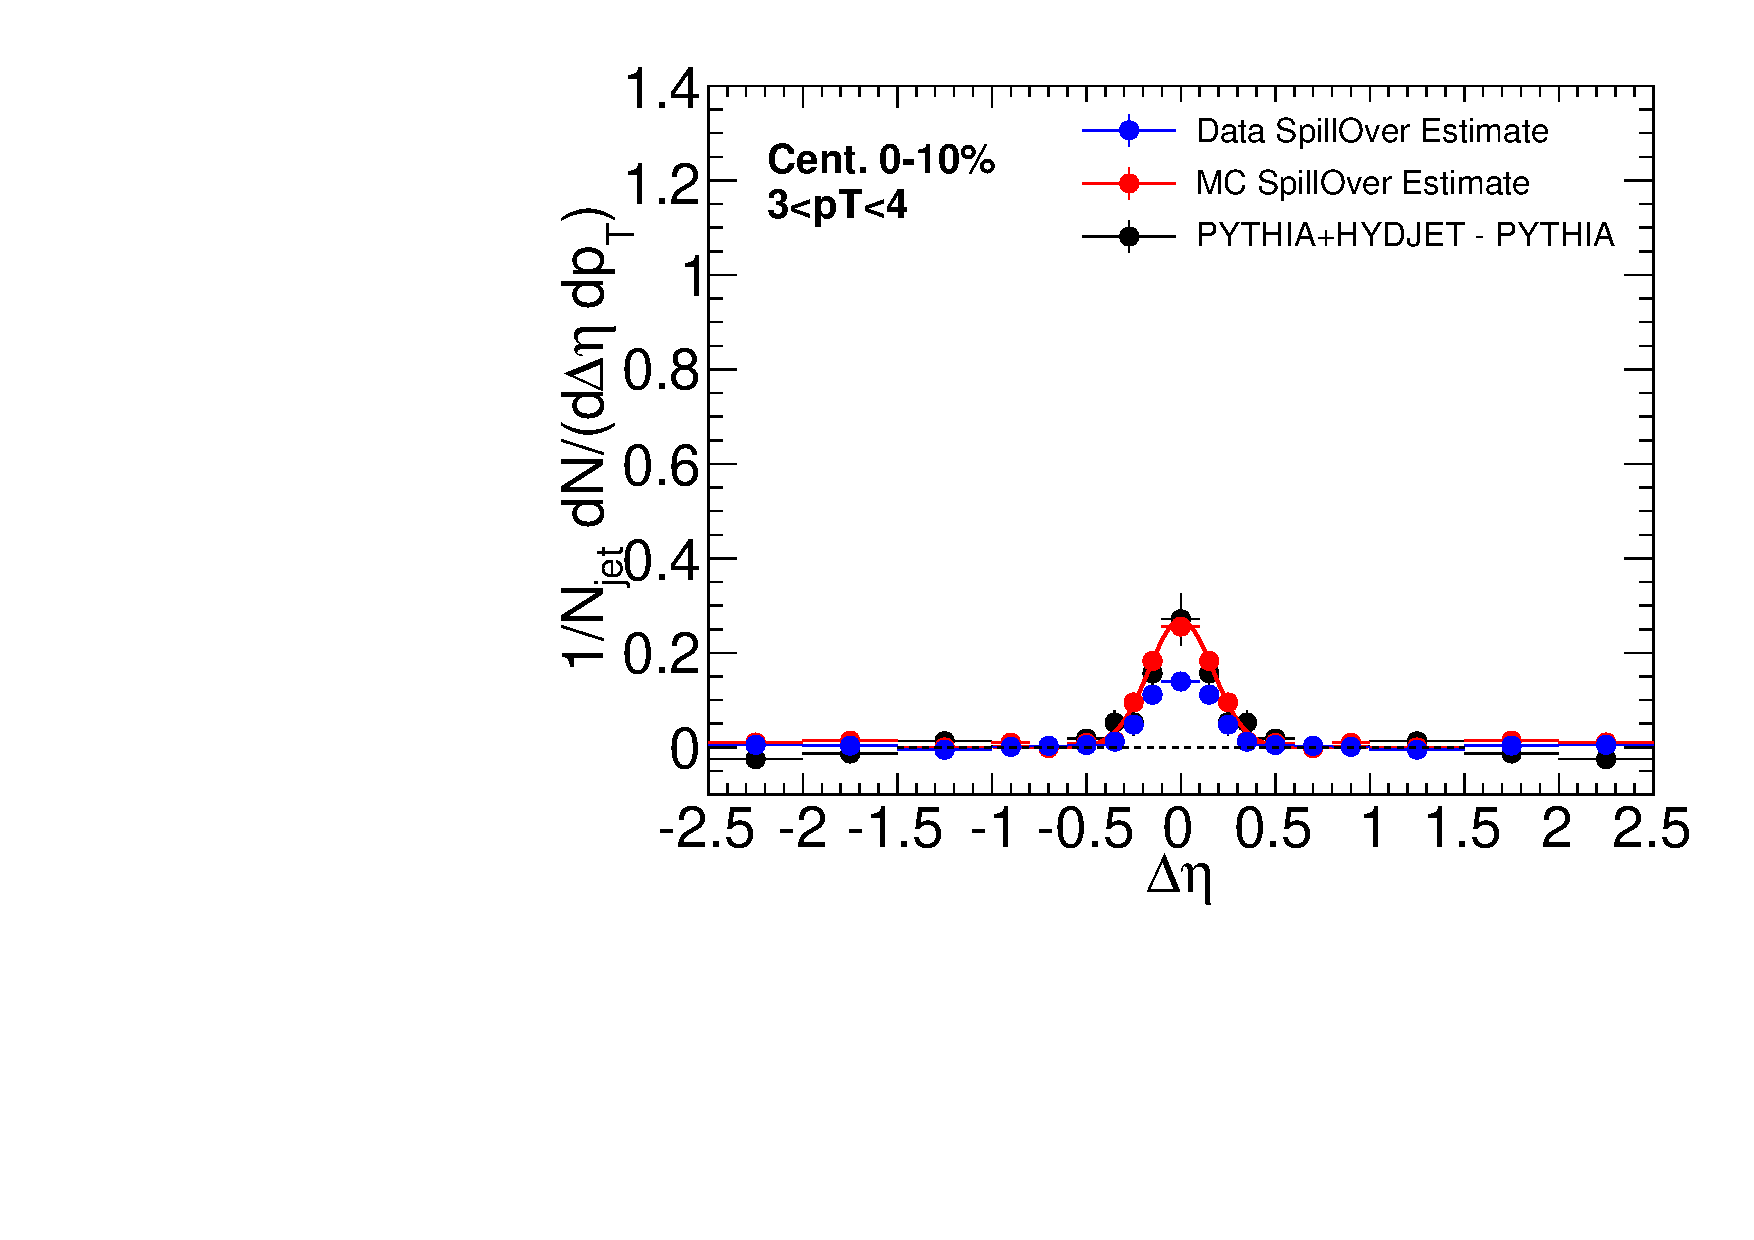
\includegraphics[width=0.49\textwidth]{figures/JFF_SpillOver/Data_Closures_TrkPt3_TrkPt4.pdf}
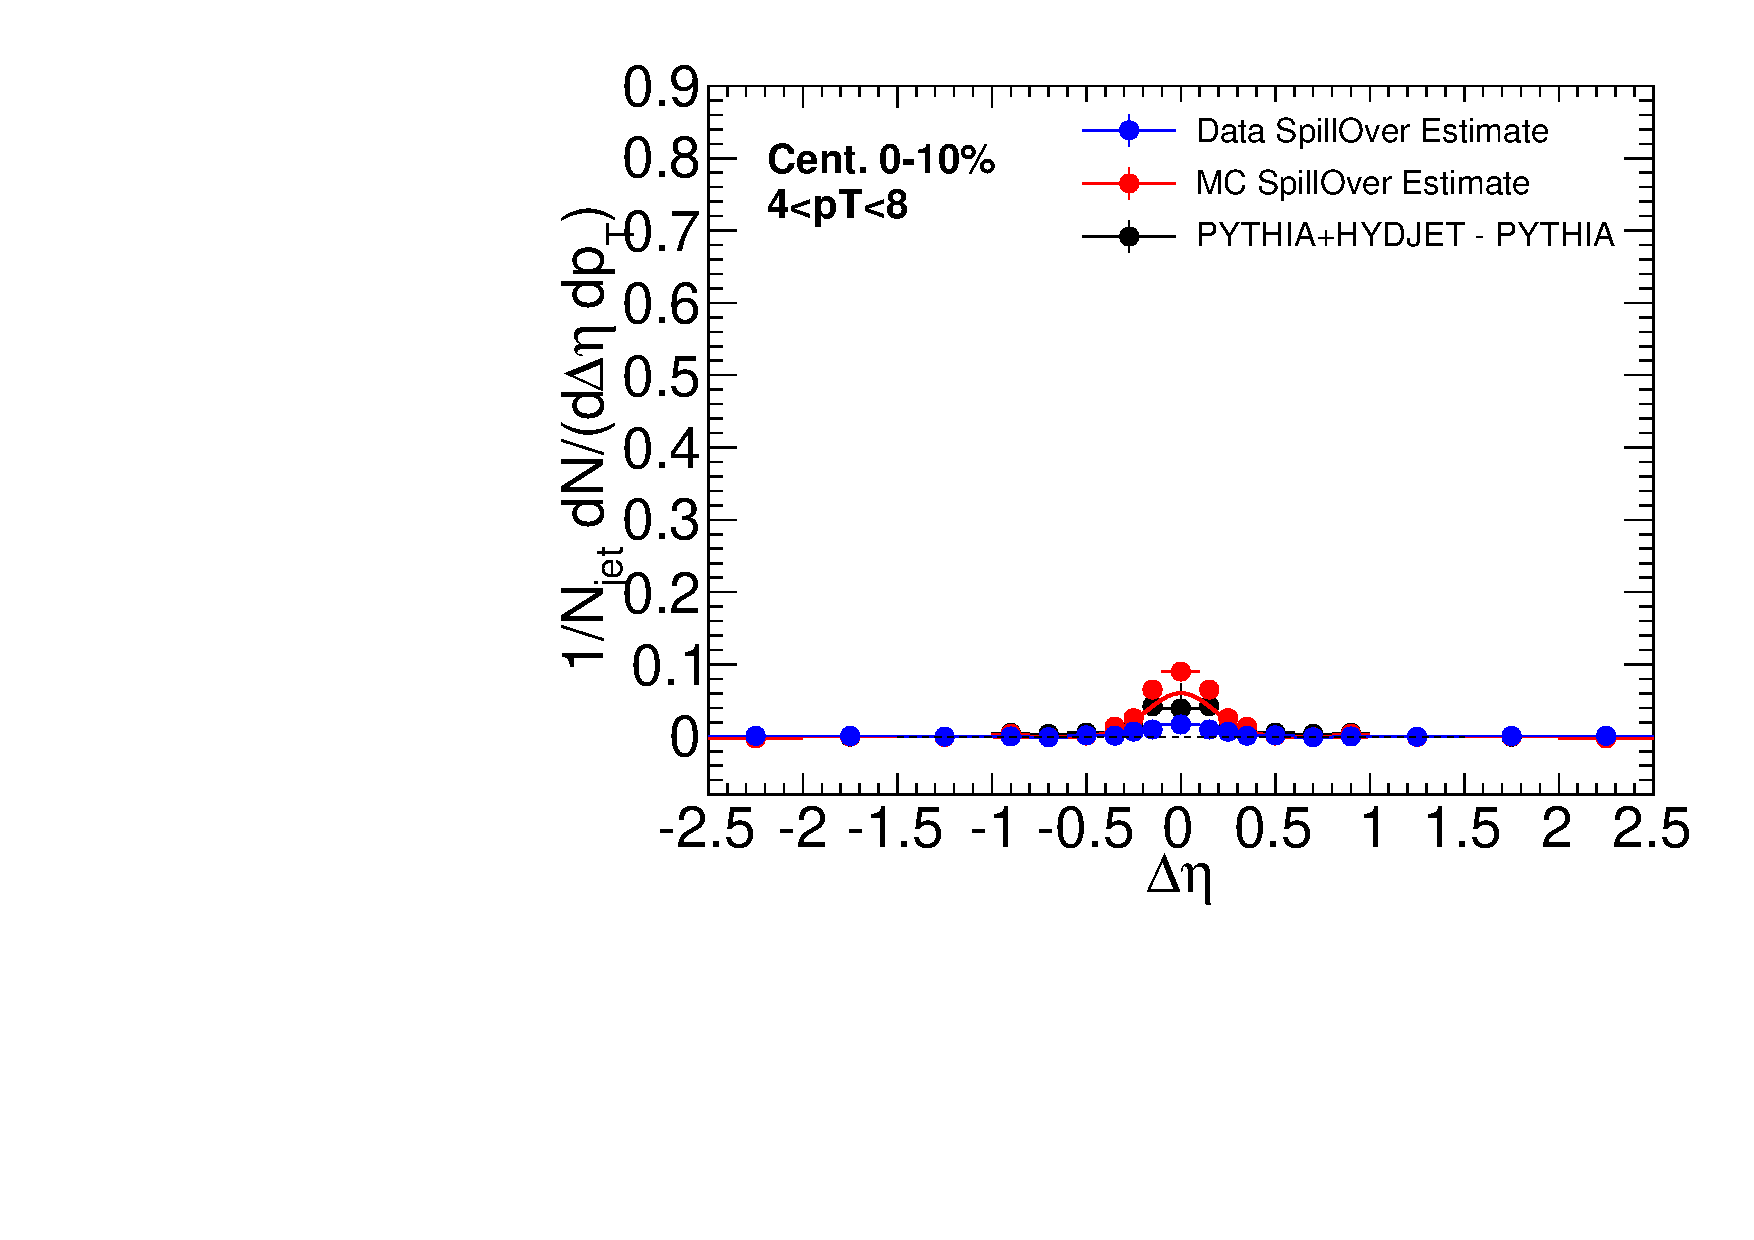
\includegraphics[width=0.49\textwidth]{figures/JFF_SpillOver/Data_Closures_TrkPt4_TrkPt8.pdf}
\caption[Data-driven check of correlated $\Delta\eta$ yields attributed to background fluctuation bias]{Correlated yield $\Delta\eta$ due to background fluctuation bias as simulated with pp jets embedded in Minimum Bias events (blue points) compared to the effect applying the same technique with {\sc pythia}  jets in {\sc hydjet}  minimum bias events, as well as in full {\sc pythia+hydjet} simulation (black points with red fit line).}
\label{fig:data_spill_bins}
\end{center}
\end{figure}
 
The background fluctuation bias could also be sensitive to the same calorimeter nonlinearity bias that necessitates fragmentation-jet energy corrections.  To study this question and validate the uncertainty associated with this correction, we separately study the effect for quark jets and gluon jets, as shown in Figure~\ref{fig:quark_gluon_closure}.  This study is limited by statistics, but deviations (or fluctuations) in the bias for quark versus gluon jets are are within the 50\% systematic uncertainty assigned.  


                  \begin{figure}[hbtp]
                  \begin{center}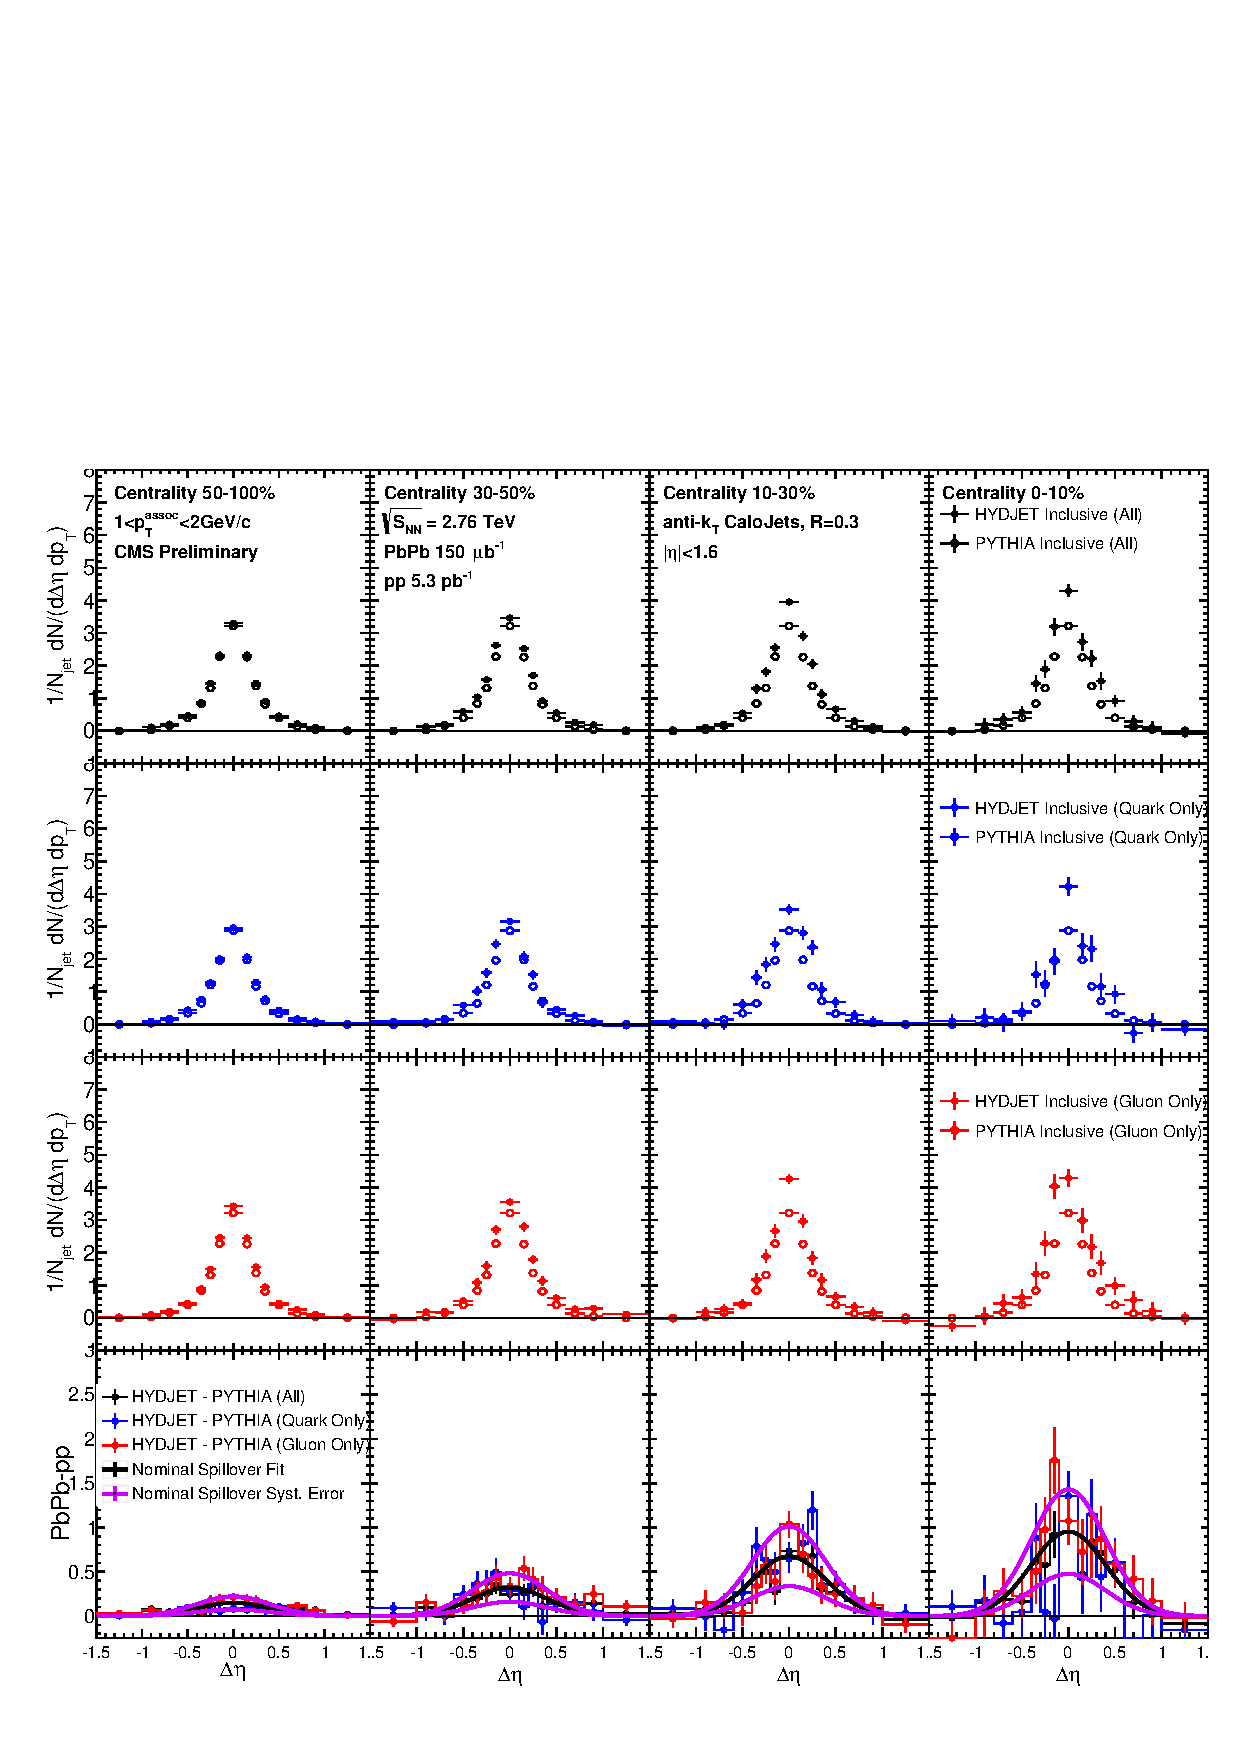
\includegraphics[width=0.99\textwidth]{figures/JFF_SpillOver/QuarkGluonComparison.pdf}
                  \caption[Comparison of background selection bias effect for quark verus gluon jets]{Comparison of magnitude of background selection bias effect for quark and gluon jets versus our nominal sample.  Jet selection is inclusive in all cases.}
                    \label{fig:quark_gluon_closure}
                    \end{center}
                    \end{figure}


                 

\clearpage

	
\subsection{Evaluation of systematic uncertainties}

A number of sources of systematic uncertainty have been discussed in presenting jet and track reconstruction and the jet-track correlation analysis procedure.  To estimate the total systematic uncertainty in these measurements, these contributions are added in quadrature.  A brief summary of all systematic uncertainty contributions, together with the procedure used to estimate their magnitude follows.  The contributions from each source (relative to jet peak signal) are summarized in Tables~\ref{tab:sys1}--\ref{tab:sys3}.

\subsubsection{Systematic uncertainties related to jet reconstruction}

Jet reconstruction-related sources of systematic uncertainty in this analysis include the two reconstruction biases as discussed above, as well uncertainty associated with the jet energy scale (JES) evaluation.  We consider three sources of uncertainty on the JES:  (1) differences in calorimeter response for quark versus gluon jets, meaning that medium-induced changes in jet flavor could result in either over-correction or under-correction of jet energy and a resulting bias in jet selection (evaluated via Monte Carlo non-closure for quark and gluon jets); (2) possible differences between data and simulation; (3) uncertainty due to quenching effects not included in our {\sc hydjet} simulation.  To evaluate how each of these sources of JES uncertainty affects final correlations, we vary jet selection threshold by the combined uncertainty, and then quantify the resulting differences in the final correlations as a measure of the combined residual JES uncertainty. Since all the measured correlations are studied per-reconstructed jets, the jet reconstruction efficiency does not contribute to the systematic uncertainty of this measurement.

\subsubsection{Systematic uncertainties related to tracking and tracking efficiency corrections}

The tracking efficiency correction uncertainty is estimated from the ratio of corrected reconstructed yields and generated yields by using generator level charged particles as a ``truth'' reference.  To account for the possible track reconstruction differences in data and simulation, a residual uncertainty in track reconstruction efficiency and fake rate corrections is also estimated.   

\subsubsection{Systematic uncertainty associated with pair acceptance correction and event decomposition}

Uncertainty arising from pair-acceptance effects is estimated by considering the sideband asymmetry after dividing by the mixed-event background.  Each sideband region of the final $\Delta\eta$ distribution ($-2.5<\Delta\eta<-1.5$ and $1.5<\Delta\eta<2.5$) is separately fit with a horizontal line after background subtraction.  The greater of these two deviations from zero is assigned as systematic error.  Uncertainties resulting from the background subtraction are determined by considering the average point-to-point deviation in two parts of the sideband region ($1.5<|\Delta\eta|<2.0$ and $2.0<|\Delta\eta|<2.5$) after background subtraction.  The derivations of both of these sources of uncertainty are illustrated in Appendix~\ref{app:err_me_bkg}.  In PbPb data this background subtraction uncertainty is greatest for the most central events (0--10\%) and the lowest track $p_{\rm T}$ bin where the background is most significant compared to the signal level, and decreases for less central collisions and for higher $p_{\rm T}$ tracks ($p_{\rm T}^{\rm trk} > 2$ GeV).  

\subsubsection{Summary of systematic uncertainties}

The contributions to total systematic uncertainty from each of the sources described above are given in Tables~\ref{tab:sys1}--\ref{tab:sys3}. Table~\ref{tab:sys1} gives uncertainty evaluations for correlation studies at 2.76 TeV, while Table~\ref{tab:sys2} gives the same for studies at 5.02 TeV.  Finally, Table~\ref{tab:sys3} gives uncertainty evaluations for balanced ($A_{\rm J} < 0.22$) and unbalanced ($A_{\rm J} > 0.22$) dijet events in momentum balance studies at 2.76 TeV.  

\begin{table}[htbp]
\begin{center}

\caption[Systematic uncertainties for particle density correlation studies at 2.76 TeV]{Systematic uncertainties in the measurement of the jet-track correlations in PbPb and pp collisions at 2.76 TeV, as percentage of the total measured correlated yield. The numbers presented in this table summarize the range of values of systematic uncertainty (as a function of $p_{\rm T}^{\rm trk}$) for different centrality bins.}
\label{tab:sys1}
\begin{tabular}{c|cccc|c}
\hline
\hline
Source & 0--10\% &  10--30\% & 30--50\% & 50--100\% &  pp \\ \hline
\hline

Background fluctuation bias             & 3--12\% & 2--7\% & 1--5\% & 0--1\% &  -- \\
Jet fragmentation function bias       & 0--2\% &    0--2\% &   0--2\% & 0--2\% &  0--2\% \\
Residual jet energy scale                                   & 3\% &    3\% &   3\% &    3\% &   3\% \\
Tracking efficiency uncertainty          & 4\% & 4\% & 4\% & 4\% &   3 \%  \\
Residual track efficiency corr.              &    5\% &    5\% &    5\% &    5\% &    5\% \\
Pair acceptance corrections                  & 5--9\% & 5--9\% & 4--8\% & 2--6\% &  2--3\% \\
Background subtraction                       & 2--5\% & 2--5\% & 2--5\% & 2--5\% &  1--2\% \\


\hline
Total                                        & 9--17\% & 9--14\% & 8--13\% & 8--10\% & 7--8\% \\

\hline


\end{tabular}
\end{center}
\end{table}


\begin{table}[htbp]
\begin{center}
	
\caption[Systematic uncertainties for particle density correlation studies at 5.02 TeV]{Systematic uncertainties in the measurement of the jet track correlations in PbPb and pp collisions at 5.02 TeV. The numbers presented in this table summarize typical range of systematic uncertainty as a function of collision centrality.  The upper limits of the cited values correspond to uncertainties at lowest $p_{\rm T}^{\rm trk}$, and uncertainties decrease with rising $p_{\rm T}^{\rm trk}$.}

\begin{tabular}{c|ccccc}
\hline
\hline
Source & 0--10\% &  10--30\% & 30--50\%& 50--100\% & ppRef \\ 
\hline
Background fluctuation bias              & 0--10\%    & 0--5\%  &        0--2\%  &       0--1\% & -- \\
Background fluctuation bias residual      & 0--2\% &       0--3\% &     0--1\% &     0--1\%&       --\\
JFF bias                                         & 3--5\%      & 3--4\% &        3--4\%&       3--4\%    &    3\% \\
Residual JES                                   & 4\% &       4\% &               4\% &            4\% &          4\% \\  
Tracking efficiency uncertainty          & 1\% &             1\%&         1\%&           1\% &        1\%  \\
Residual tracking efficiency              &    5\% &                5\%&      5\%&            5\% &         5\% \\
Pair-acceptance corrections              & 1--5\% &      1--4\% &     1--4\% &       1--4\% &       1--2\% \\
Event decomposition                     & 1--9\% &       0--4\% &     0--4\% &     0--3\%&       0--3\% \\
\hline
Total                                        & 7--16\%     & 7--11\%     & 7--9\%  & 7--9\% &        7--8\% \\
\hline
\hline
\end{tabular}
\label{tab:sys2}
\end{center}
\end{table}





\begin{table}[htbp]

\begin{center}
\caption[Systematic uncertainties for balanced and unbalanced dijets in transverse momentum distribution studies at 2.76 TeV]{This table summarizes the systematic uncertainties in the measurement of the $p_{\rm T}^{\rm trk}$ correlations in PbPb and pp collisions at 2.76 TeV. Upper and lower limits are shown as a function of collision centrality.  Upper values correspond to the uncertainties at lowest $p_{\rm T}^{\rm trk}$.}
\label{tab:sys3}
\begin{tabular}{c|ccccc}
\hline
\hline

Source & 0--30\% &   30--50\% & 50--100\% & pp \\ \hline
\hline
Balanced jet selection ($A_{\rm J} < 0.22$):\\
\hline
Background fluctuations                       & 1--8\%  & 1--3\% & 0--1\% & -- \\
JFF bias and jet swapping               & 0--2\%  &   0--2\% & 0--2\% &    0--2\% \\
Residual JES                                   & 3\% &      3\% &    3\% &    3\% \\
Tracking efficiency         & 4\%  & 4\% & 4\% & 3 \%  \\
Residual track efficiency corr.              &    5\%  &    5\% &    5\% &    5\% \\
Pair acceptance corrections                  & 5--9\%  & 4--8\% & 2--6\% & 2--3\% \\
Event decomposition                      & 2--5\% & 2--5\% & 2--5\% & 1--2\% \\
\hline
Total                                        & 9--15\%  & 8--13\% & 8--10\% & 7--8\% \\
\hline
\hline
Unbalanced jet selection ($A_{\rm J} > 0.22$):\\
\hline
Background fluctuations                       & 1--10\% &  1--5\% & 0--2\% & -- \\
JFF bias and jet swapping               & 0--2\% &      0--2\% & 0--2\% &    0--2\% \\
Residual JES                                   & 3\% &     3\% &    3\% &    3\% \\
Tracking efficiency           & 4\% & 4\% & 4\% & 3 \%  \\
Residual track efficiency corr.              &    5\% &    5\% &    5\% &    5\% \\
Pair acceptance corrections                  & 5--9\%  & 4--8\% & 2--6\% & 2--3\% \\
Event decomposition                    & 2--5\% &  2--5\% & 2--5\% & 1--2\% \\
\hline
Total                                        & 9--16\%  & 8--13\% & 8--10\% & 7--8\% \\

\hline
\hline

\end{tabular}
\end{center}
\end{table}


